\chapter{R{\'e}nyi Divergence Variational Inference}
\label{chap:vrbound}

% **************************** Define Graphics Path **************************
\ifpdf
    \graphicspath{{Chapter4/Figs/Raster/}{Chapter4/Figs/PDF/}{Chapter4/figs/}}
\else
    \graphicspath{{Chapter4/Figs/Vector/}{Chapter4/figs/}}
\fi


We have discussed in the last chapter a class of EP-like algorithms, which unifies EP, SEP and VI from an algorithmic point of view. Approximate inference is also widely used as a sub-routine in approximate maximum likelihood algorithms and those used for model selections. Historically, VI has received most attentions in this regard. This is mainly because VI has elegant and useful theoretical properties, such as the fact that it proposes a lower-bound of the log-model evidence. 
%
On the other hand, as discussed in the previous chapter, the underlying objective function of SEP is unknown and might not even exist. Even the EP energy itself, although often providing more accurate approximations, has no bounding guarantees \citep{cunningham:gaussianEP2011}. These undesirable issues make EP-like algorithms less appropriate for model selection and approximate MLE. 

To (partially) address these issues, in this chapter we will present a new class of variational inference method using a variant of the $\alpha$-divergences called R{\'e}nyi divergence. We will develop both lower- and upper-bounds to the marginal likelihood, and draw connections to SEP and Black-box-$\alpha$ (introduced by us in \cite{hernandez-lobato:bbalpha2016} but not included in the thesis). This framework is also computationally compelling for Bayesian deep learning, as it is compatible with gradient descent methods (unlike SEP methods which use moment matching). These favourable features are demonstrated with examples including variational auto-encoders and Bayesian neural networks. Throughout the development we will also discuss some theoretical properties of Monte Carlo approximations and data sub-sampling.

%\section{R{\'e}nyi divergences for variational inference}
\label{sec:vrbound_all}

% general idea
%
%%%%%% why VR bound %%%%%%%%
In this section we try to provide a unified framework from an energy function perspective that encompasses a number of recent advances in variational methods, and we hope our effort could potentially motivate new algorithms in the future. This is done by extending traditional VI to R{\'e}nyi's $\alpha$-divergence \cite{renyi:divergence1961}, a rich family that includes many well-known divergences as special cases. After reviewing useful properties of R{\'e}nyi divergences and the VI framework, we make the following contributions:

\begin{itemize}
 \item We introduce the \emph{variational R{\'e}nyi bound} (VR) as an extension of VI/VB. We then discuss connections to existing approaches, including VI/VB, VAE, IWAE \cite{burda:iwae2016}, SEP and BB-$\alpha$, thereby showing the richness of this new family of variational methods.
 %\vspace{-0.03in} 
 \item We develop an optimisation framework for the VR bound. An analysis of the bias introduced by stochastic approximation is also provided with theoretical guarantees and empirical results.
 %\vspace{-0.03in} 
 \item We propose a novel approximate inference algorithm called \emph{VR-max} as a new special case. Evaluations on VAEs and Bayesian neural networks show that this new method is often comparable to, or even better than, a number of the state-of-the-art variational methods.
\end{itemize}

%%%%%%%%% trend of approximate inference %%%%%%%%%%%

\textbf{Remark.} Recent advances of approximate inference follow three major trends. These developments are rather separated and little work has been done to understand their connections, until this section was presented as a conference paper.

First, scalable methods, e.g.~stochastic variational inference (SVI) \cite{hoffman:svi2013} and stochastic expectation propagation (SEP)/AEP \cite{barthelme:aep2015}, have been developed for datasets comprising millions of datapoints. Recent approaches \cite{broderick:stream2013, gelman:dep2014, xu:sms2014} have also applied variational methods to coordinate parallel updates arising from computations performed on chunks of data.

Second, Monte Carlo methods and black-box inference techniques have been deployed to assist variational methods, e.g.~see \cite{paisley:bbvi2012, salimans:reparam2013, ranganath:bbvi2014, kucukelbir:advi2015} for VI and BB-$\alpha$ for EP. They all proposed ascending the Monte Carlo approximated variational bounds to the log-likelihood using noisy gradients computed with automatic differentiation tools.

Third, tighter variational lower-bounds have been proposed for (approximate) MLE. The importance weighted auto-encoder (IWAE) \cite{burda:iwae2016} improved upon the variational auto-encoder (VAE) \cite{kingma:vae2014, rezende:vae2014} framework, by providing tighter lower-bound approximations to the log-likelihood using importance sampling. 
\section{R{\'e}nyi's $\alpha$-divergence}

\label{sec:chap4_vrbound_renyi_divergence}
We first review R{\'e}nyi's $\alpha$-divergence \citep{renyi:divergence1961, van_erven:renyi2014}. R{\'e}nyi's $\alpha$-divergence, defined on $\{\alpha: \alpha > 0, \alpha \neq 1, |\mathrm{D}_{\alpha}^{R}| < +\infty \}$, measures the ``closeness'' of two distributions $p$ and $q$ on a random variable $\bm{\theta} \in \Theta$:
\begin{equation}
\label{eq:renyi_divergence}
\mathrm{D}_{\alpha}^{R} [p || q] = \frac{1}{\alpha - 1} \log \int p(\bm{\theta})^{\alpha} q(\bm{\theta})^{1 - \alpha} d \mu.
\end{equation}
Here the constraint $|D^{R}_{\alpha}[p||q]| < +\infty$ is crucial for rewriting the divergence as the expectation under $p$ or $q$ (i.e. to change the measure from $d\mu$ to $dP$ or $dQ$), i.e. 
$$D_{\alpha}[p||q] = \frac{1}{\alpha - 1} \log \mathbb{E}_{p} \left[ \left( \frac{p(\bm{\theta})}{q(\bm{\theta})}   \right)^{\alpha - 1} \right] = \frac{1}{\alpha - 1} \log \mathbb{E}_{q} \left[ \left( \frac{p(\bm{\theta})}{q(\bm{\theta})}   \right)^{\alpha} \right],$$
since it is possible that the definition (\ref{eq:renyi_divergence}) is infinity but one of the above expectations is finite. In the following we will use $d\mu = d\bm{\theta}$ w.l.o.g.

The definition is extended to $\alpha = 0, 1, +\infty$ by continuity. We note that when $\alpha \rightarrow 1$ the Kullback-Leibler (KL) divergence is recovered, which plays a crucial role in machine learning and information theory. Some other special cases are presented in Table \ref{tab:renyi_example}. The method proposed in this work also considers $\alpha \leq 0$ (although (\ref{eq:renyi_divergence}) is no longer a divergence for these $\alpha$ values), and we include from \cite{van_erven:renyi2014} some useful properties for forthcoming derivations.
%
\begin{prop}
(Monotonicity) R{\'e}nyi's $\alpha$-divergence definition (\ref{eq:renyi_divergence}), extended to negative $\alpha$, is \textbf{continuous} and \textbf{non-decreasing} on $\alpha \in \{\alpha: -\infty < \mathrm{D}_{\alpha}^{R} < +\infty \}$.
\label{prop:renyi_divergence}
\end{prop}
%
\begin{prop}
(Skew symmetry) For $\alpha \not\in \{0, 1\}$, 
$
\mathrm{D}_{\alpha}^{R} [p || q] = \frac{\alpha}{1 - \alpha} \mathrm{D}_{1 - \alpha}^{R} [q || p].
$
This implies $\mathrm{D}_{\alpha}^{R} [p || q] \leq 0$ for $\alpha < 0$. For the limiting case $\mathrm{D}_{-\infty}^{R} [p || q] = -\mathrm{D}_{+\infty}^{R} [q || p]$.
\label{prop:skew_symmetry}
\end{prop}
%
%
\begin{table}[t]
  \centering
  \caption{Special cases in the R{\'e}nyi divergence family.}
  \renewcommand{\arraystretch}{1.2}
  \label{tab:renyi_example}
  \begin{tabular}{ccl}
  	\toprule
    $\alpha$ & Definition & Notes\\
    \hline
    $\alpha \rightarrow 1$ & $\int p(\bm{\theta}) \log \frac{p(\bm{\theta})}{q(\bm{\theta})} d \bm{\theta}$ & 
    \begin{tabular}{@{}l@{}} \emph{Kullback-Leibler (KL) divergence}, \\ used in VI ($\mathrm{KL}[q||p]$) and EP ($\mathrm{KL}[p||q]$) \end{tabular} \\
    %
    $\alpha = 0.5$ & $-2 \log (1 - \mathrm{Hel}^2[p||q])$ & function of the square \emph{Hellinger distance}\\
    %
    $\alpha \rightarrow 0$ & $-\log \int_{p(\bm{\theta}) > 0} q(\bm{\theta}) d\bm{\theta}$ & 
    \begin{tabular}{@{}l@{}} zero when $\mathrm{supp}(q) \subseteq \mathrm{supp}(p)$ \\ (not a divergence) \end{tabular} \\
    %
    $\alpha = 2$ & $-\log (1 - \chi^2[p||q])$ & 
    \begin{tabular}{@{}l@{}} proportional to the $\chi^2$-divergence \end{tabular} \\
    %
    $\alpha \rightarrow +\infty$ & $\log \max_{\bm{\theta} \in \Theta} \frac{p(\bm{\theta})}{q(\bm{\theta})}$ &
    \begin{tabular}{@{}l@{}} \emph{worst-case regret} in \\ \emph{minimum description length principle} \citep{grunwald:mdl2007}\end{tabular} \\
    \bottomrule
  \end{tabular}
  %\vspace{-0.1in}
\end{table}
%
A critical question that is still in active research is how to choose a divergence in this rich family to obtain optimal solution for a particular application, an issue which is discussed in Section \ref{sec:chap4_vrbound_opt_mc}.
\section{Variational R{\'e}nyi bound}
\label{sec:vr_bound}
Recall from previous section that the family of R{\'e}nyi divergences includes the KL divergence. Perhaps variational free-energy approaches can be generalised to the R{\'e}nyi case? Consider approximating the exact posterior $p(\mparam|\mathcal{D})$ by minimizing R{\'e}nyi's $\alpha$-divergence $\mathrm{D}_{\alpha}^{R}[q(\mparam) || p(\mparam | \mathcal{D})]$ for some selected $\alpha > 0$.
%
Now we consider the equivalent optimisation problem 
$$\max_{q \in \mathcal{Q}} \quad  \log p(\mathcal{D}) - \mathrm{D}_{\alpha}^{R}[q(\mparam) || p(\mparam | \mathcal{D})],$$
when $\alpha \neq 1$, the objective can be rewritten as
\begin{equation}
\begin{aligned}
\mathcal{L}_{\alpha}(q; \mathcal{D}) := & \log p(\mathcal{D}) - \mathrm{D}_{\alpha}^{R}[q(\mparam) || p(\mparam | \mathcal{D})] \\
= & \log p(\mathcal{D}) - \frac{1}{\alpha - 1} \log \mathbb{E}_{q} \left[ \left( \frac{q(\mparam) p(\mathcal{D})}{p(\mparam, \mathcal{D})} \right)^{\alpha - 1} \right] \\
= & \frac{1}{1 - \alpha} \log \mathbb{E}_{q} \left[ \left( \frac{p(\mparam, \mathcal{D})}{q(\mparam)} \right)^{1 - \alpha} \right].
\end{aligned}
\label{eq:chap4_vrbound_exact_bound}
\end{equation}
%
We name this new objective the \emph{variational R{\'e}nyi (VR) bound}. Importantly the above definition can be extended to $\alpha \leq 0$, and the following theorem is a direct result of Proposition \ref{prop:renyi_divergence}.
\begin{theorem}
\label{thm:chap4_vrbound_alpha_vi}
The objective $\mathcal{L}_{\alpha}(q; \mathcal{D})$ is \textbf{continuous} and \textbf{non-increasing} on $\alpha \in \{\alpha: |\mathcal{L}_{\alpha}| < +\infty \}$. Especially for all $0 < \alpha_{+} < 1$ and $\alpha_{-} < 0$,
\begin{equation*}
\mathcal{L}_{\text{VI}}(q; \mathcal{D}) = \lim_{\alpha \rightarrow 1} \mathcal{L}_{\alpha}(q; \mathcal{D}) 
 \leq \mathcal{L}_{\alpha_{+}}(q; \mathcal{D}) \leq \mathcal{L}_{0}(q; \mathcal{D}) \leq \mathcal{L}_{\alpha_{-}}(q; \mathcal{D})
\end{equation*}
Also $\mathcal{L}_{0}(q; \mathcal{D}) = \log p(\mathcal{D})$ if and only if the support $ \mathrm{supp}(p(\mparam|\mathcal{D})) \subseteq  \mathrm{supp}(q(\mparam)) $.
\end{theorem}
%
Theorem \ref{thm:chap4_vrbound_alpha_vi} indicates that the VR bound can be useful for model selection by sandwiching the marginal likelihood with bounds computed using positive and negative $\alpha$ values, which we leave to future work. In particular $\mathcal{L}_{0} = \log p(\mathcal{D})$ under the mild assumption that $q$ is supported where the exact posterior is supported. This assumption holds for many commonly used distributions, e.g.~Gaussians are supported on the entire space, and in the following we assume that this condition is satisfied. 

\vspace{1em}
\begin{tcolorbox}
\textbf{Remark} (on marginal likelihood estimation)\textbf{.}
Though not fully discussed in this thesis, it is worth highlighting here the importance of robust marginal likelihood estimation, and thus the usefulness of sandwiching estimates (with both a lower- and an upper-bound). \citet{dieng:chi2016} applied the VR upper-bound to a number of real-world tasks. \cite{grosse:bidirectional2015, grosse:bidirectional2016} proposed bi-directional Monte Carlo method that can be viewed as computing the VR bounds with a sequence of proposal distributions, aiming at reducing the mismatch between $q$ and $p$ thus improving the Monte Carlo estimates. \cite{wu:quantitative2017} applied this idea to perform the first attempt of robust predictive log-likelihood estimation for VAEs and generative adversarial networks (GANs) \citep{goodfellow:gan2014}.   
\end{tcolorbox}
%

\subsection{Mean-field approximation revisited}
\label{sec:chap4_mean_field}

We revisit in the following the mean-field approximation by optimising the VR bound, with Bayesian linear regression as an illustrating example. Recall the mean-field approximation factorises over the components of $\mparam = (\theta_1, ..., \theta_D)$: $q(\mparam) = \prod_{i} q_i(\theta_i)$. Re-writing the VR bound (\ref{eq:chap4_vrbound_exact_bound}), we have
\begin{equation*}
\begin{aligned}
\mathcal{L}_{\alpha}(q; \mathcal{D}) &= \frac{1}{1 - \alpha} \log \int \prod_i q_i(\theta_i)  \left( \frac{p(\mparam, \mathcal{D})}{\prod_i q_i(\theta_i)} \right)^{1 - \alpha} d\mparam \\
&= \frac{1}{1 - \alpha} \log \int q_j(\theta_j)^{\alpha} \left( \int \prod_{i \neq j} q_i(\theta_i)  \left( \frac{p(\mparam, \mathcal{D})}{\prod_{i \neq j} q_i(\theta_i)} \right)^{1 - \alpha} d\mparam_{\neq j} \right) d\theta_j \\
&:= \frac{1}{1 - \alpha} \log \int q_j(\theta_j)^{\alpha} \tilde{p}_j(\theta_j)^{1 - \alpha} d\theta_j + \text{const},
\end{aligned}
\end{equation*}
where $\tilde{p}_j(\theta_j)$ denote the ``marginal'' distribution satisfying
\begin{equation*}
\log \tilde{p}_j(\theta_j) = \frac{1}{1 - \alpha} \log \int \prod_{i \neq j} q_i(\theta_i)  \left( \frac{p(\mparam, \mathcal{D})}{\prod_{i \neq j} q_i(\theta_i)} \right)^{1 - \alpha} d\mparam_{\neq j} + \text{const}.
\end{equation*}
Now maximising the VR bound (when $\alpha > 0$, and for $\alpha < 0$ we minimise the bound) is equivalent to minimising $\mathrm{D}_{\alpha}^{R}[q_j||\tilde{p}_j]$ (for $\alpha > 0$, and when $\alpha < 0$ we minimise $\mathrm{D}_{1 - \alpha}^{R}[\tilde{p}_j||q_j]$), which means $\log q_j(\theta_j) = \log \tilde{p}_j(\theta_j) + \text{const}$ is the only global optimum of the mean-field approximation procedure. One can verify that when $\alpha \rightarrow 1$ it recovers the traditional variational mean-field approximation (see Section \ref{sec:chap2_mean_field_vi})
\begin{equation*}
\lim_{\alpha \rightarrow 1} \log \tilde{p}_j(\theta_j) = \int \prod_{i \neq j} q_i(\theta_i) \log p(\mparam, \mathcal{D}) d\mparam_{\neq j} + \text{const},
\end{equation*}
and when $\alpha \rightarrow 0$ the fixed point equation returns the exact marginal of the posterior distribution:\footnote{This is \emph{not} the unique fixed point of $\lim_{\alpha \rightarrow 0} \mathcal{L}_{\alpha} = \mathcal{L}_0$, since $\mathcal{L}_0 = \text{const}$ when $q$ has full support.} 
$$\lim_{\alpha \rightarrow 0} \tilde{p}_j(\theta_j) = p(\theta_j |\mathcal{D}).$$

Now consider Bayesian linear regression with 2-D input $\bm{x}$ and 1-D output $y$, as an example:
\begin{equation*}
\mparam \sim \mathcal{N}(\mparam; \bm{\mu}_0, \bm{\Lambda}_0^{-1}), \quad 
y|\bm{x} \sim \mathcal{N}(y; \mparam^T \bm{x}, \sigma^2).
\end{equation*}
Given the observations $\mathcal{D} = \{\bm{x}_n, y_n \}$, the posterior distribution of $\mparam$ can be computed analytically as $p(\mparam|\mathcal{D}) = \mathcal{N}(\mparam; \bm{\mu}, \bm{\Lambda}^{-1})$ with $\bm{\Lambda} = \bm{\Lambda}_0 + \frac{1}{\sigma^2} \sum_n \bm{x}_n \bm{x}_n^T$ and $\bm{\Lambda} \bm{\mu} = \bm{\Lambda}_0 \bm{\mu}_0 + \frac{1}{\sigma^2} \sum_n y_n \bm{x}_n$. To see how the mean-field approach works we explicitly write down the elements of the posterior parameters
\begin{equation*}
\bm{\mu} = \begin{pmatrix} \mu_1 \\ \mu_2 \end{pmatrix}, \quad
\bm{\Lambda} = \begin{pmatrix} \Lambda_{11} & \Lambda_{12} \\ \Lambda_{21} & \Lambda_{22} \end{pmatrix}, 
\quad \Lambda_{12} = \Lambda_{21},
\end{equation*}
and define $q_i(\theta_i) = \mathcal{N}(\theta_i; m_i, \lambda_i^{-1})$ as a univariate Gaussian distribution. Then
\begin{equation*}
\begin{aligned}
\log q_1 &= \frac{1}{1 - \alpha} \log \int q_2(\theta_2)  \left( \frac{p(\mparam, \mathcal{D})}{q_2(\theta_2)} \right)^{1 - \alpha} d\theta_2 + \text{const} \\
&= \frac{1}{1 - \alpha} \log \int \exp \left[ -\frac{1 - \alpha}{2} (\mparam - \bm{\mu})^T \bm{\Lambda} (\mparam - \bm{\mu}) - \frac{\alpha}{2} \lambda_2 (\theta_2 - m_2)^2 \right] d\theta_2 + \text{const} \\
&= \frac{1}{1 - \alpha} \log \int \mathcal{N}(\mparam; \bm{\mu}, \tilde{\bm{\Sigma}}) d\theta_2 + \text{const} \\
&= \log \mathcal{N}(\theta_1; m_1, \lambda^{-1}) + \text{const}
\end{aligned}
\end{equation*}
where the new mean $m_1$ and the precision $\lambda_1$ satisfies
\begin{equation*}
\begin{aligned}
m_1 = \mu_1 + C_1(\mu_2 - m_2), \quad C_1 = \frac{\alpha \lambda_2 \Lambda_{12}}{(1 - \alpha) |\bm{\Lambda}| + \alpha \lambda_2 \Lambda_{11}}, \\
\lambda_1 = \Lambda_{11} - (1 - \alpha) \Lambda_{12} ((1 - \alpha) \Lambda_{22} + \alpha \lambda_2)^{-1} \Lambda_{21}.
\end{aligned}
\end{equation*}
One can derive the terms $m_2$ and $C_2$ for $q_2$ in the same way, and show that $\bm{m} = \bm{\mu}$ is the only stable fixed point of this iterative update. So we have $q_1 = \mathcal{N}(\theta_1; \mu_1, \lambda_1^{-1})$, and similarly $q_2 = \mathcal{N}(\theta_1; \mu_2, \lambda_2^{-1})$ with $\lambda_2 = \Lambda_{22} - (1 - \alpha) \Lambda_{21} ((1 - \alpha) \Lambda_{11} + \alpha \lambda_1)^{-1} \Lambda_{12}$. In this example $\lambda_1$, $\lambda_2$ are feasible for all $\alpha$, and solving the fixed point equations, finally we have the stable fixed point as
\begin{equation*}
\lambda_1 = \rho_{\alpha} \Lambda_{11}, \quad \lambda_2 = \rho_{\alpha} \Lambda_{22}, \quad 
\rho_{\alpha} = \frac{1}{2 \alpha} \left[ (2\alpha - 1) + \sqrt{1 - \frac{4\alpha (1 - \alpha) \Lambda_{12}^2}{\Lambda_{11} \Lambda_{22}}} \right].
\end{equation*}
The other solution for the quadratic formula is eliminated since it violates the assumptions that $\lambda_1 > 0$ (when $0 < \alpha < 1$) and $|\mathcal{L}_{\alpha}| < +\infty$ (when $\alpha < 0$ or $\alpha > 1$, since it requires $|\alpha \text{diag}(\bm{\lambda}) + (1 - \alpha)\bm{\Lambda}| > 0$). Thus the stable fixed point in this case is unique.

One can show that $\lim_{\alpha \rightarrow 1} \lambda_1 = \Lambda_{11}$ (the precision of the conditional distribution $p(\theta_1 | \theta_2, \data)$), $\lim_{\alpha \rightarrow 0} \lambda_1 = \Lambda_{11} - \Lambda_{12} \Lambda_{22}^{-1} \Lambda_{21}$ (the precision of the marginal distribution $p(\theta_1|\data)$), and $\lim_{\alpha \rightarrow \pm \infty} \lambda_1 = \Lambda_{11} \pm |\Lambda_{12}| \sqrt{\Lambda_{11} \Lambda_{22}^{-1}}$ (similar results for $\lambda_2$). Also $\rho_{\alpha}$ is continuous and non-decreasing in $\alpha$. This means one can interpolate between mass-covering ($\alpha \rightarrow -\infty$) and zero-forcing ($\alpha \rightarrow +\infty$, when using uni-modal approximations it is usually called mode-seeking) behaviour by increasing $\alpha$ values. 

We visualise the analytical results for Bayesian linear regression in Figure \ref{fig:chap4_vrbound_linear_regression_posterior} and  \ref{fig:chap4_vrbound_linear_regression_energy}. First as predicted, increasing $\alpha$ returns more confident estimate. Also notice that $\alpha \rightarrow +\infty$ (in cyan) returns non-zero uncertainty estimates (although it is more over-confident than VI) which is different from the maximum a posteriori (MAP) method that only returns a point estimate. Second, setting $\alpha = 0.0$ (in green) returns $q(\mparam) = \prod_i p(\theta_i|\mathcal{D})$ and the exact marginal likelihood $\log p(\mathcal{D})$ (Figure \ref{fig:chap4_vrbound_linear_regression_energy}). Also the approximate MLE is less biased for $\alpha = 0.5$ (in blue) since now the tightness of the bound is less hyper-parameter dependent.

\begin{figure}[t]
 \centering
 \subfigure[Approximated posterior.]{
 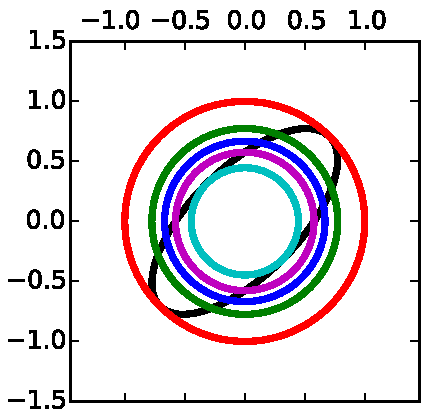
\includegraphics[width=0.24\linewidth]{Chapter4/figs/approx.pdf}
 \label{fig:chap4_vrbound_linear_regression_posterior}}
 \hspace{0.5in}
 \subfigure[Hyper-parameter optimisation.]{
 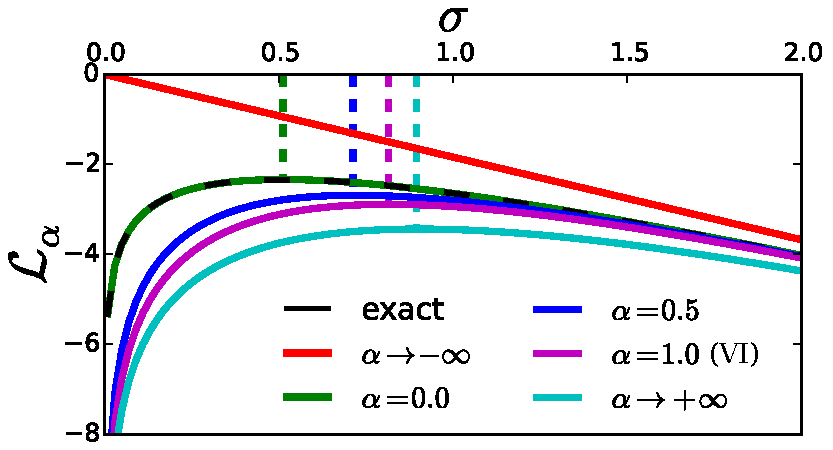
\includegraphics[width=0.45\linewidth]{Chapter4/figs/log_evidence.pdf}
 \label{fig:chap4_vrbound_linear_regression_energy}}
 \caption{Mean-Field approximation for Bayesian linear regression (with one-sigma contours). C.f. Figure \ref{fig:chap2_mean_field}. In this case $\bm{\varphi} = \sigma$ the observation noise variance. As expected when $\alpha = 0$ the resulting bound coincides with the exact log marginal (see the green-black curve). The bound is tight as $\sigma \rightarrow +\infty$, biasing the VI solution to large $\sigma$ values.}
\end{figure}


\subsection{Monte Carlo approximation of the VR bound}
\label{sec:chap4_vrbound_sampling}

Although we have seen some nice properties of the VR bound optimisation through the mean-field approximation example, we also note that when $\alpha \neq 1$, the VR bound is usually just as intractable as the marginal likelihood for many other useful models. Also Theorem \ref{thm:chap4_vrbound_alpha_vi} suggests that the VR bound is to be minimised when $\alpha < 0$, which performs disastrously in MLE context.
%
 As we shall see, these issues are addressed by the MC approximation that we will be developing as follows, under certain conditions. Therefore, MC-VR can be applied to precisely the same set of models as MC-VI \citep{paisley:bbvi2012, salimans:reparam2013, ranganath:bbvi2014, kucukelbir:advi2015}.

Consider learning a latent variable model with MLE as a running example, where the model is specified by a conditional distribution $p(\bm{x}|\z, \bm{\varphi})$ and a prior $p(\z| \bm{\varphi})$ on the latent variable $\z$. Examples include latent variable models treated by the variational auto-encoder (VAE) approach \citep{kingma:vae2014, rezende:vae2014} that parametrises the likelihood with a (deep) neural network. MLE requires $\log p(\bm{x})$ which is obtained by marginalising out $\z$ and is often intractable, so the VR bound is considered as an alternative optimisation objective. However instead of using exact bounds, a simple Monte Carlo (MC) method is deployed, which uses a finite number of samples $\z_k \sim q(\z|\bm{x}), k = 1, ..., K$ to approximate the VR bound $\mathcal{L}_{\alpha} \approx \hat{\mathcal{L}}_{\alpha, K}$:
\begin{equation}
\label{eq:sampling_estimate}
\hat{\mathcal{L}}_{\alpha, K}(q; \bm{x}) = \frac{1}{1 - \alpha} \log \frac{1}{K} \sum_{k=1}^K \left[\left( \frac{p(\z_k, \bm{x})}{q(\z_k|\bm{x})} \right)^{1 - \alpha} \right].
\end{equation}
The importance weighted auto-encoder (IWAE) \citep{burda:iwae2016} is a special case of this framework with $\alpha = 0$ and $K < +\infty$. But unlike traditional VI, here the MC approximation is biased. Fortunately we can characterise the bias by the following theorems (proofs provided in Appendix \ref{sec:appendix_proof_chap4}).
%
%
%%%%% theorem %%%%%
\begin{theorem}
\label{thm:chap4_vrbound_sampling_bound}
Assume $\mathbb{E}_{\{\z_k\}_{k=1}^K} [ |\hat{\mathcal{L}}_{\alpha, K}(q; \bm{x})| ] < + \infty$ and $|\mathcal{L}_{\alpha}| < +\infty$. Then $\mathbb{E}_{\{\z_k\}_{k=1}^K} [ \hat{\mathcal{L}}_{\alpha, K}(q; \bm{x}) ]$ as a function of $\alpha \in \mathbb{R}$ and $K \geq 1$ is: \\
1) \textbf{non-decreasing} in $K$ for fixed $\alpha \leq 1$, and \textbf{non-increasing} in $K$ for fixed $\alpha \geq 1$; \\
2) $\mathbb{E}_{\{\z_k\}_{k=1}^K} [ \hat{\mathcal{L}}_{\alpha, K}(q; \bm{x}) ] \rightarrow \mathcal{L}_{\alpha}$ as $K \rightarrow +\infty$; \\
3) \textbf{continuous} and \textbf{non-increasing} in $\alpha$ with fixed $K$.
\end{theorem}

%%%%%% corollary %%%%%
\begin{corollary}
\label{thm:chap4_vrbound_alpha_k_existence}
For finite $K$, either $\mathbb{E}_{\{\z_k\}_{k=1}^K} [ \hat{\mathcal{L}}_{\alpha, K}(q; \bm{x}) ] < \log p(\bm{x})$ for all $\alpha$, or there exists $\alpha_K \leq 0$ such that $\mathbb{E}_{\{\z_k\}_{k=1}^K} [ \hat{\mathcal{L}}_{\alpha_K, K}(q; \bm{x}) ] = \log p(\bm{x})$ and $\mathbb{E}_{\{\z_k\}_{k=1}^K} [ \hat{\mathcal{L}}_{\alpha, K}(q; \bm{x}) ] > \log p(\bm{x})$ for all $\alpha < \alpha_K$. Also $\alpha_K$ is \textbf{non-decreasing} in $K$ if exists, with $\lim_{K \rightarrow 1} \alpha_K = -\infty$ and $\lim_{K \rightarrow +\infty} \alpha_K = 0$.
\end{corollary}
%%%%%%%%%%%%%%%%

%
The intuition behind the theorems is visualised in Figure \ref{fig:chap4_vrbound_divergence_sampling}. By definition, the exact VR bound is a lower-bound or upper-bound of $\log p(\bm{x})$ when $\alpha > 0$ or $\alpha < 0$, respectively. However the MC approximation $\mathbb{E}[\hat{\mathcal{L}}_{\alpha, K}]$ biases the estimate towards $\mathcal{L}_{\text{VI}}$, where the MC approximation of the bound can be improved using more samples. Thus for finite samples and under mild conditions, negative alpha values can potentially be used to improve the accuracy of the approximation, although the MC approximation for these alpha values is no longer guaranteed to be an upper bound.
%
Figure \ref{fig:chap4_vrbound_divergence_simulation} shows an empirical evaluation by computing the exact and the MC approximation of the R{\'e}nyi divergence. In this example $p$, $q$ are 2-D Gaussian distributions with $\bm{\mu}_p = [0, 0]$, $\bm{\mu}_q = [1, 1]$ and $\bm{\Sigma}_p = \bm{\Sigma}_q = \bm{I}$. The sampling procedure is repeated 200 times to estimate the expectation. Clearly for $K = 1$ it is equivalent to an unbiased estimate of the KL-divergence for all $\alpha$ (even though now the estimation is biased for $\mathrm{D}_{\alpha}^{R}$). For $K > 1$ and $\alpha < 1$, the MC method under-estimates the VR bound, and the bias decreases with increasing $K$. For $\alpha > 1$ the inequality is reversed also as predicted.


\begin{figure*}[t]
 \centering
 \subfigure[MC approximated VR bounds.]{
 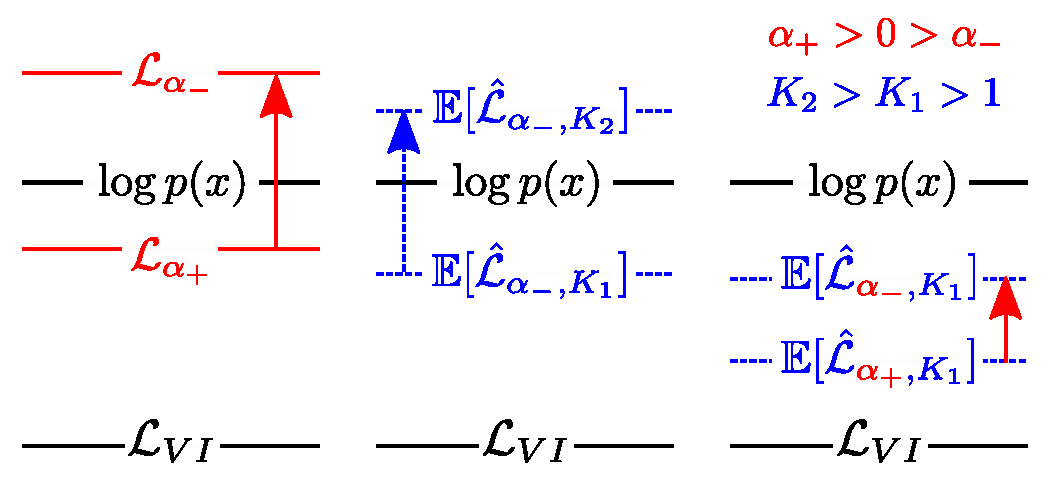
\includegraphics[width=0.6\linewidth]{sampling_bound_full.pdf}
 \label{fig:chap4_vrbound_divergence_sampling}}
 \hspace{0.1in}
 \subfigure[Simulated MC approximations.]{
 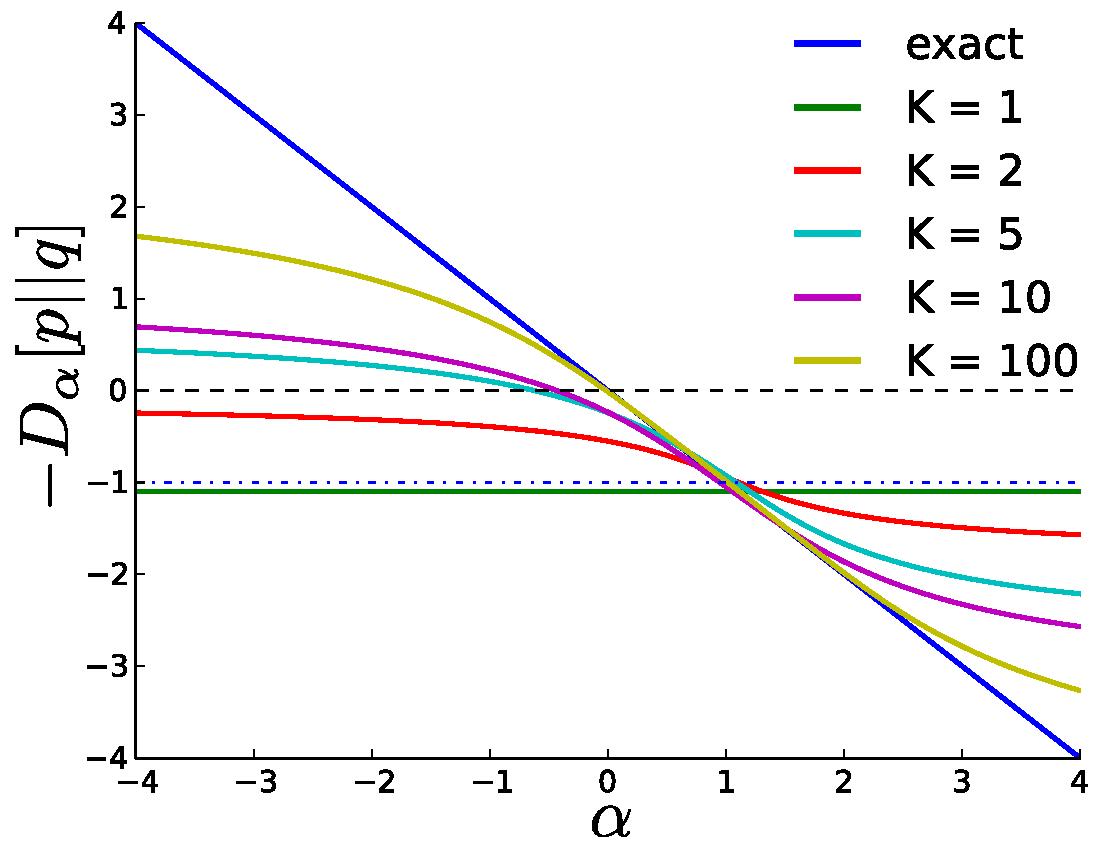
\includegraphics[width=0.34\linewidth]{divergence_sampling.pdf}
 \label{fig:chap4_vrbound_divergence_simulation}}
 \vspace{-0.1in}
 \caption{(a) An illustration for the bounding properties of MC approximations to the VR bounds (non-increasing in $\alpha$ and non-decreasing in $K$ when $\alpha \leq 1$). (b) The bias of the MC approximation, where the dash-dotted line on top of the green line ($K=1$) is the analytical value of $-\mathrm{KL}[p||q]$. Best viewed in colour and see the main text for details.}
\end{figure*}
%%%%%%%%%%%%%%%%%%%%
\subsection{A unified implementation with the reparameterisation trick}

Readers may have noticed that $\mathcal{L}_{\text{VI}}$ has a different form compared to $\mathcal{L}_{\alpha}$ with $\alpha \neq 1$. In this section we show how to unify the implementation for all finite $\alpha$ settings using the \emph{reparameterisation trick} \citep{salimans:reparam2013, kingma:vae2014} as an example. This trick assumes the existence of the mapping $\bm{\theta} = g_{\bm{\phi}}(\bm{\epsilon})$, where the distribution of the noise term $\bm{\epsilon}$ satisfies $q(\bm{\theta}) d\bm{\theta} = p(\bm{\epsilon}) d\bm{\epsilon}$. Then the expectation of a function $F(\bm{\theta})$ over distribution $q(\bm{\theta})$ can be computed as
%
$\mathbb{E}_{q(\bm{\theta})} [F(\bm{\theta})] = \mathbb{E}_{p(\bm{\epsilon})} [F(g_{\bm{\phi}}(\bm{\epsilon}))].$
%
One prevalent example is the Gaussian reparameterisation: $\bm{\theta} \sim \mathcal{N}(\bm{\mu}, \Sigma) \Rightarrow \bm{\theta} = \bm{\mu} + \Sigma^{ \frac{1}{2} } \bm{\epsilon}$, with $\bm{\epsilon} \sim \mathcal{N}(\bm{0}, I)$. 
%
Now we apply the reparameterisation trick to the VR bound
%
\begin{equation}
\mathcal{L}_{\alpha}(q_{\bm{\phi}}; \bm{x}) = \frac{1}{1 - \alpha} \log \mathbb{E}_{\bm{\epsilon}} \left[\left( \frac{p(g_{\bm{\phi}}(\bm{\epsilon}) , \bm{x})}{q(g_{\bm{\phi}}(\bm{\epsilon}))} \right)^{1 - \alpha} \right].
\end{equation}
%
For notational ease we also write $g_{\bm{\phi}} = g_{\bm{\phi}}(\bm{\epsilon})$. Then the gradient of the VR bound w.r.t.~$\bm{\phi}$ (similar for $\bm{\varphi}$) is
\begin{equation}
\begin{aligned}
\nabla_{\bm{\phi}} \mathcal{L}_{\alpha}(q_{\bm{\phi}}; \bm{x}) 
&= \frac{1}{1 - \alpha} \nabla_{\bm{\phi}} \log \mathbb{E}_{\bm{\epsilon}} \left[ \left( \frac{p(g_{\bm{\phi}}, \bm{x})}{q(g_{\bm{\phi}})} \right)^{1 - \alpha} \right] \\
&= \frac{1}{1 - \alpha} \left( \mathbb{E}_{\bm{\epsilon}} \left[ \left( \frac{p(g_{\bm{\phi}}, \bm{x})}{q(g_{\bm{\phi}})} \right)^{1 - \alpha} \right] \right)^{-1} \mathbb{E}_{\bm{\epsilon}} \left[ \nabla_{\bm{\phi}} \left( \frac{p(g_{\bm{\phi}}, \bm{x})}{q(g_{\bm{\phi}})} \right)^{1 - \alpha} \right] \\
&= \frac{1}{1 - \alpha} \left( \mathbb{E}_{\bm{\epsilon}} \left[ \left( \frac{p(g_{\bm{\phi}}, \bm{x})}{q(g_{\bm{\phi}})} \right)^{1 - \alpha} \right] \right)^{-1} \mathbb{E}_{\bm{\epsilon}} \left[ \left( \frac{p(g_{\bm{\phi}}, \bm{x})}{q(g_{\bm{\phi}})} \right)^{1 - \alpha} \nabla_{\bm{\phi}} (1 - \alpha) \log \frac{p(g_{\bm{\phi}}, \bm{x})}{q(g_{\bm{\phi}})} \right] \\
&= \mathbb{E}_{\bm{\epsilon}} \left[ w_{\alpha}(\bm{\epsilon}; \bm{\phi}, \bm{x}) \nabla_{\bm{\phi}} \log \frac{p(g_{\bm{\phi}}, \bm{x})}{q(g_{\bm{\phi}})} \right].
\end{aligned}
\label{eq:chap4_vrbound_gradient_reparam}
\end{equation}
%
where $w_{\alpha}(\bm{\epsilon}; \bm{\phi}, \bm{x}) = \left( \frac{p(g_{\bm{\phi}}(\bm{\epsilon}), \bm{x})}{q(g_{\bm{\phi}}(\bm{\epsilon}))} \right)^{1 - \alpha} \bigg/ \mathbb{E}_{\bm{\epsilon}} \left[ \left( \frac{p(g_{\bm{\phi}}(\bm{\epsilon}), \bm{x})}{q(g_{\bm{\phi}}(\bm{\epsilon}))} \right)^{1 - \alpha} \right]$ denotes the normalised importance weight. 
%
One can show that this recovers the the stochastic gradients of $\mathcal{L}_{\text{VI}}$ by setting $\alpha = 1$ in (\ref{eq:chap4_vrbound_gradient_reparam}) since now $w_{1}(\bm{\epsilon}; \bm{\phi}, \bm{x}) = 1$, which means the resulting algorithm unifies the computation for all finite $\alpha$ settings. For MC approximations, we use $K$ samples to approximately compute the weight $\hat{w}_{\alpha, k}(\bm{\epsilon}_k; \bm{\phi}, \bm{x}) \propto \left( \frac{p(g_{\bm{\phi}}(\bm{\epsilon}_k), \bm{x})}{q(g_{\bm{\phi}}(\bm{\epsilon}_k))} \right)^{1 - \alpha}$, $k = 1, ..., K$, and the stochastic gradient becomes
\begin{equation}
\nabla_{\bm{\phi}} \hat{\mathcal{L}}_{\alpha, K}(q_{\bm{\phi}}; \bm{x}) 
= \sum_{k=1}^K \left[ \hat{w}_{\alpha, k}(\bm{\epsilon}_k; \bm{\phi}, \bm{x}) \nabla_{\bm{\phi}} \log \frac{p(g_{\bm{\phi}}(\bm{\epsilon}_k), \bm{x})}{q(g_{\bm{\phi}}(\bm{\epsilon}_k))} \right].
\end{equation}
When $\alpha = 1$, $\hat{w}_{1, k}(\bm{\epsilon}_k; \bm{\phi}, \bm{x}) = 1/K$, and it recovers the stochastic gradient VI method \citep{kingma:vae2014}.

To speed-up learning \citet{burda:iwae2016} suggested back-propagating only one sample $\bm{\epsilon}_j$ with $j \sim p_j = \hat{w}_{\alpha, j}$, which can be easily extended to our framework. Importantly, the use of different $\alpha < 1$ indicates the degree of emphasis placed upon locations where the approximation $q$ under-estimates $p$, and in the extreme case $\alpha \rightarrow -\infty$, the algorithm chooses the sample that has the \emph{maximum} unnormalised importance weight. 
%
We name this approach \emph{VR-max} and summarise it and the general case in Algorithm \ref{alg:vr_max}. 
%
Note that VR-max (and VR-$\alpha$ with $\alpha < 0$ and MC approximations) does \emph{not} minimise $\mathrm{D}_{1-\alpha}^{R}[p||q]$. It is true that $\mathcal{L}_{\alpha} \geq \log p(\bm{x})$ for negative $\alpha$ values. However Corollary \ref{thm:chap4_vrbound_alpha_k_existence} suggests that the tightest MC approximation for given $K$ has non-positive $\alpha_K$ value, or might not even exist. Furthermore the optimal $\alpha_K$ value becomes more negative as the mismatch between $q$ and $p$ increases, e.g.~the VAE uses a uni-modal $q$ distribution to approximate the typically multi-modal exact posterior.



\begin{figure}[!t]
% UGLY USE OF \vspace & \hspace follows
\begin{minipage}[b]{0.55\linewidth}
\centering
\begin{algorithm}[H] 
\caption{One gradient step for VR-$\alpha$/VR-max with single backward pass. Here $\hat{w}(\bm{\epsilon}_k; \bm{x})$ short-hands $\hat{w}_{0, k}(\bm{\epsilon}_k; \bm{\phi}, \bm{x})$ in the main text.} \small
\label{alg:vr_max} 
\begin{algorithmic}[1] 
	\STATE given the current datapoint $\bm{x}$, sample \\$\bm{\epsilon}_1, ..., \bm{\epsilon}_K \sim p(\bm{\epsilon})$
	\STATE for $k = 1, ..., K$, compute the unnormalised weight \\
	$\log \hat{w}(\bm{\epsilon}_k; \bm{x}) = \log p(g_{\bm{\phi}}(\bm{\epsilon}_k), \bm{x}) - \log q(g_{\bm{\phi}}(\bm{\epsilon}_k)|\bm{x})$
	\STATE choose the sample $\bm{\epsilon}_{j}$ to back-propagate: \\
	if $|\alpha| < \infty$: $j \sim p_k$ where $p_k \propto \hat{w}(\bm{\epsilon}_k; \bm{x})^{1 - \alpha}$ \\
	if $\alpha = -\infty$: $j = \argmax_{k} \log \hat{w}(\bm{\epsilon}_k; \bm{x})$ 
	\STATE return the gradients $\nabla_{\bm{\phi}} \log \hat{w}(\bm{\epsilon}_{j}; \bm{x})$
\end{algorithmic}
\end{algorithm}
\end{minipage}
%
\hfill
\begin{minipage}[b]{0.4\linewidth}
\centering
 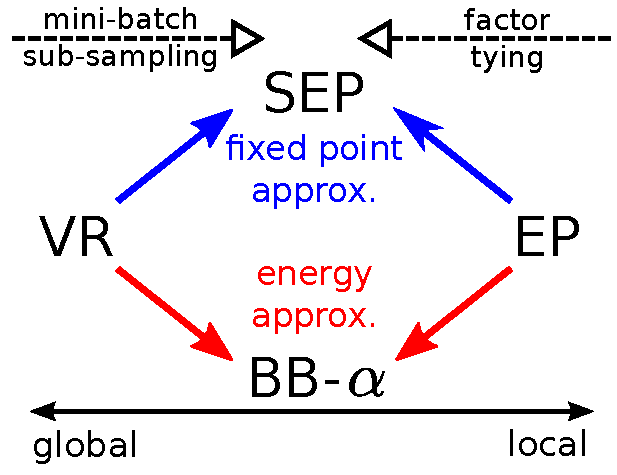
\includegraphics[width=0.9\linewidth]{vr_ep_relationship.pdf} 
 \vspace{-0.1in}
 \captionof{figure}{Connecting local and global divergence minimisation.}
 \label{fig:vr_ep_relationship}
\end{minipage}
%\quad
%
\end{figure}


%%%%%%%%%%%%%%
\subsection{Stochastic approximation for large-scale learning}
\label{sec:chap4_vrbound_large_scale_learning}
VR bounds can also be applied to full Bayesian inference with posterior approximation. However for large datasets full batch learning is very inefficient. Mini-batch training is non-trivial here since the VR bound cannot be represented by the expectation of a datapoint-wise loss, except when $\alpha = 1$ (VI). This section introduces two proposals for mini-batch training, and interestingly, this recovers two existing algorithms that were motivated from a different perspective.
%
In the following we define the (geometric) ``average likelihood'' $\bar{f}_{\mathcal{D}}(\bm{\theta}) = [\prod_{n=1}^N p(\bm{x}_n|\bm{\theta})]^{\frac{1}{N}}$. Hence the joint distribution can be rewritten as $p(\bm{\theta}, \mathcal{D}) = p_0(\bm{\theta}) \bar{f}_{\mathcal{D}}(\bm{\theta})^N$. Also for a mini-batch of $M$ datapoints $\mathcal{S} = \{\bm{x}_{n_1}, ..., \bm{x}_{n_M} \} \sim \mathcal{D}$, we define the ``subset average likelihood'' $\bar{f}_{\mathcal{S}}(\bm{\theta}) = [\prod_{m=1}^M p(\bm{x}_{n_m}|\bm{\theta})]^{\frac{1}{M}}$.

The first proposal considers \emph{fixed point approximations} with mini-batch sub-sampling. It first derives the fixed point conditions for the variational parameters (e.g.~the natural parameters of $q$) using the exact VR bound (\ref{eq:chap4_vrbound_exact_bound}), then designs an iterative algorithm using those fixed point equations, but with $\bar{f}_{\mathcal{D}}(\bm{\theta})$ replaced by $\bar{f}_{\mathcal{S}}(\bm{\theta})$.
%
The second proposal also applies this subset average likelihood approximation idea, but directly to the VR bound (\ref{eq:chap4_vrbound_exact_bound}) (so this approach is named \emph{energy approximation}):
\begin{equation}
\label{eq:alpha_vi_approx}
\tilde{\mathcal{L}}_{\alpha}(q; \mathcal{S}) 
	= \frac{1}{1 - \alpha} \log \mathbb{E}_{q} \left[ \left( \frac{p_0(\bm{\theta}) \bar{f}_{\mathcal{S}}(\bm{\theta})^N} {q(\bm{\theta})} \right)^{1 - \alpha} \right].
\end{equation}
%
Now we demonstrate with detailed derivations that fixed point approximation returns stochastic EP (SEP, see Chapter \ref{chap:factor_tying}) , and black box alpha (BB-$\alpha$) \citep{hernandez-lobato:bbalpha2016} corresponds to energy approximation. We derive the results in exponential family context, but in general these two principles of stochastic approximation also apply. Note that both methods use Minka's $\alpha$-divergence, and for clear distinction here we use $\beta$ instead to denote the corresponding $\alpha$ values for Minka's definition, and hence the two algorithms are returned respectively by taking $M = 1$ and $\alpha = 1 - \beta/N$.

Precisely, we assume the posterior approximation is defined as $q(\bm{\theta}) = \frac{1}{Z_q} p_0(\bm{\theta}) t(\bm{\theta})^N$.
Often $t(\bm{\theta})$ is chosen to have an exponential family form $t(\bm{\theta}) \propto \exp \left[ \langle \bm{\lambda}, \bm{\Phi}(\bm{\theta}) \rangle \right]$ with $\bm{\Phi}(\bm{\theta})$ denoting the sufficient statistic. Then picking $\alpha = 1 - \beta/N$, $\beta \neq 0$, we obtain the exact VR bound (by pulling out the normalising constant $Z_q$) as
\begin{equation}
\mathcal{L}_{\alpha}(q; \mathcal{D}) = \log Z_q + \frac{N}{\beta} \log \mathbb{E}_{q} \left[ \left( \frac{ \bar{f}_{\mathcal{D}}(\bm{\theta})} {t(\bm{\theta})} \right)^{\beta} \right].
\label{eq:vr_bound_sa_exact}
\end{equation}

The first proposal considers deriving the exact fixed point conditions, then approximating them with mini-batch sub-sampling. In our example the exact fixed point condition for the variational parameters $\bm{\lambda}$ is
\begin{equation}
\nabla_{\bm{\lambda}} \mathcal{L}_{\alpha}(q; \mathcal{D}) = 0 \quad \Rightarrow \quad \mathbb{E}_{q}[\bm{\Phi}(\bm{\theta})] = \mathbb{E}_{\tilde{p}_{\alpha}}[\bm{\Phi}(\bm{\theta})],
\end{equation} 
with the tilted distribution defined as 
$$\tilde{p}_{\alpha}(\bm{\theta}) \propto q(\bm{\theta})^{\alpha}p_0(\bm{\theta})^{1 - \alpha} \bar{f}_{\mathcal{D}}(\bm{\theta})^{N(1 - \alpha)} \propto p_0(\bm{\theta}) t(\bm{\theta})^{N - \beta} \bar{f}_{\mathcal{D}}(\bm{\theta})^{\beta}.$$ 
Now given a mini-batch of datapoints $\mathcal{S}$, the moment matching update can be approximated by replacing $\bar{f}_{\mathcal{D}}(\bm{\theta})$ with $\bar{f}_{\mathcal{S}}(\bm{\theta}) = [\prod_{m=1}^M p(\bm{x}_{n_m}|\bm{\theta})]^{\frac{1}{M}}$. More precisely, each iteration we sample a subset of data $\mathcal{S} = \{\bm{x}_{n_1}, ..., \bm{x}_{n_M} \} \sim \mathcal{D}$, and compute the new update for $\bm{\lambda}$ by first computing $\tilde{p}_{\alpha, \mathcal{S}}(\bm{\theta}) \propto p_0(\bm{\theta}) t(\bm{\theta})^{N - \beta} \bar{f}_{\mathcal{S}}(\bm{\theta})^{\beta}$ then taking $\mathbb{E}_{q}[\bm{\Phi}(\bm{\theta})] \leftarrow \mathbb{E}_{\tilde{p}_{\alpha, \mathcal{S}}}[\bm{\Phi}(\bm{\theta})]$. This method returns SEP when $M = 1$, i.e.~in each iteration only one datapoint is sampled to update the approximate posterior. Using larger mini-batch size $M > 1$ returns SDEP (see Section \ref{sec:chap3_sep_dep}) and in this case further approximation might be required to compute the fixed point iterative updates.

%
The second proposal also applies this subset average likelihood approximation idea, but directly to the VR bound (\ref{eq:vr_bound_sa_exact}), with $\mathbb{E}_{\mathcal{S}}$ denoting the expectation over mini-batch sub-sampling:
\begin{equation}
\mathbb{E}_{\mathcal{S}} \left[ \tilde{\mathcal{L}}_{\alpha}(q; \mathcal{S}) \right] = \log Z_q + \frac{N}{\beta} \mathbb{E}_{\mathcal{S}} \left[ \log \mathbb{E}_{q} \left[ \left( \frac{ \bar{f}_{\mathcal{S}}(\bm{\theta})} {t(\bm{\theta})} \right)^{\beta} \right] \right].
\label{eq:vr_bound_sa_approx}
\end{equation}
It recovers the energy function of BB-$\alpha$ when $M=1$. Note that the original BB-$\alpha$ algorithm uses an adapted form of Amari's $\alpha$-divergence, and the $\alpha$ value in the BB-$\alpha$ algorithm corresponds to $\beta$ in our exposition. Now the gradient of this approximated energy function becomes
\begin{equation}
\nabla_{\bm{\lambda}} \mathbb{E}_{\mathcal{S}} \left[ \tilde{\mathcal{L}}_{\alpha}(q; \mathcal{S}) \right] = N (\mathbb{E}_{q}[\bm{\Phi}(\bm{\theta})] - \mathbb{E}_{\mathcal{S}} \mathbb{E}_{\tilde{p}_{\alpha, \mathcal{S}}}[\bm{\Phi}(\bm{\theta})]).
\end{equation}
%
We also provide a characterisation of the energy approximation (\ref{eq:vr_bound_sa_approx}) by the following theorem, with a proof presented in Appendix \ref{sec:appendix_proof_chap4}.
%
\begin{theorem}
\label{thm:chap4_vrbound_stochastic_approx}
If the approximate distribution $q(\bm{\theta})$ is Gaussian $\mathcal{N}(\bm{\mu}, \bm{\Sigma})$, and the likelihood functions has an exponential family form $p(\bm{x}|\bm{\theta}) = \exp [\langle \bm{\theta}, \bm{\Phi}(\bm{x}) \rangle - A(\bm{\theta})]$, then for $\alpha \leq 1$ and $r > 1$ the stochastic approximation is bounded by
\begin{equation*}
\mathbb{E}_{\mathcal{S}} [\tilde{\mathcal{L}}_{\alpha}(q; \mathcal{S})] \leq \mathcal{L}_{1 - (1 - \alpha)r}(q; \mathcal{D}) + \frac{N^2(1-\alpha) r}{2(r - 1)}  \mathrm{tr}(\bm{\Sigma} \mathrm{Cov}_{\mathcal{S} \sim \mathcal{D}}( \bar{\bm{\Phi}}_{\mathcal{S}})).
\end{equation*}
\end{theorem}

The following corollary is a direct result of Theorem \ref{thm:chap4_vrbound_stochastic_approx} applied to BB-$\alpha$. Note here we follow the convention of BB-$\alpha$ to use $M = 1$ and overload the notation $\alpha = \beta$ and $\mathcal{L}_{BB-\alpha}(q; \mathcal{D}) = \mathbb{E}_{\{  \bm{x}_n\}} \left[ \tilde{\mathcal{L}}_{1 - \alpha/N}(q; \{ \bm{x}_n \}) \right]$.
\begin{corollary}
Assume the approximate posterior and the likelihood functions satisfy the assumptions in Theorem \ref{thm:chap4_vrbound_stochastic_approx}, then for $\alpha > 0$ and $r > 1$, the black-box alpha energy function is upper-bounded by
\begin{equation*}
\mathcal{L}_{BB-\alpha}(q; \mathcal{D}) \leq \mathcal{L}_{1 - \frac{\alpha r}{N}}(q; \mathcal{D}) + \frac{N \alpha r}{2(r - 1)}  \mathrm{tr}(\bm{\Sigma} \mathrm{Cov}_{\mathcal{D}}(\bm{\Phi})).
\end{equation*}
\end{corollary} 

It is interesting that both SEP and BB-$\alpha$ were originally proposed to approximate (power) EP \citep{minka:ep2001, minka:powerep2004}, which usually minimises $\alpha$-divergences \emph{locally}, and considers $M=1$, $\alpha \in [1 - 1/N, 1)$ and exponential family distributions. These approximations were performed by factor tying, which significantly reduces the memory overhead of full EP and makes both SEP and BB-$\alpha$ scalable to large datasets just as is the case for SVI. The new derivation provides a theoretical justification from an energy perspective, and also sheds lights on the connections between \emph{local} and \emph{global} divergence minimisations as depicted in Figure \ref{fig:vr_ep_relationship}. Note that all these methods recover SVI when $\alpha \rightarrow 1$, in which global and local divergence minimisation are equivalent. Also these results suggest again (but from a different perspective) that, recent attempts of distributed posterior approximation (by carving up the dataset into pieces with $M > 1$ \citep{gelman:dep2014, xu:sms2014}) can be extended to both SEP and BB-$\alpha$.

SEP is arguably better justified since it returns the exact posterior if the approximation family $\mathcal{Q}$ is large enough to include the correct solution, just like VI and VR computed on the whole dataset. BB-$\alpha$ might still be biased even in this scenario. However, BB-$\alpha$ is much simpler to implement since the energy function can be optimised with stochastic gradient descent. Indeed BB-$\alpha$ considers the same black-box approach as used for VI, by computing a stochastic estimate of the energy function then using automatic differentiation tools to obtain the gradients. 

%
%Monte Carlo methods can also be applied to both proposals. For SEP the moment computation can be approximated with MCMC \citep{gelman:dep2014, xu:sms2014}. For BB-$\alpha$ one can show in the same way as to prove Theorem \ref{thm:chap4_vrbound_sampling_bound} that simple MC approximation in expectation lower-bounds the BB-$\alpha$ energy when $\alpha \leq 1$. 

%%%% discussion on MC approximation %%%%
\subsection{Optimisation issues with $\alpha$-divergences and MC approximations}
\label{sec:chap4_vrbound_opt_mc}

It is in general an outstanding research question on how to select the divergence measure for a particular machine learning problem. In our case this corresponds to selecting the $\alpha$ value. Also an approximate inference algorithm can be evaluated with different performance measures, and it is generally impossible to find a single $\alpha$ value that returns the best performance on all evaluations. Thus we only present the evaluation in test error and test log-likelihood in the experiments, and use them to select the $\alpha$ values empirically. 

We discuss two conjectures to explain the difficulty of selecting $\alpha$ in the Bayesian neural network experiments presented in later sections. The first conjecture is that zero-forcing algorithms ($\alpha \geq 1$) tend to favour minimising the test error, while mass-covering methods ($\alpha < 1$) tend to improve the test log-likelihood. However zero-forcing methods can fail as they might miss an important mode due to local optima. Similarly mass-covering methods can be pathological if the exact posterior includes modes that are very far away from each other. Furthermore, the form of the posterior will change with the number of observed datapoints $N$, so the ``optimal'' setting of $\alpha$ for a fixed task may change with $N$. 

The second conjecture states that the MC approximation complicates the selection of $\alpha$, since it favours zero-forcing (because of the bias introduced). For example, in order to maximise the quantity of the MC approximation the algorithm need to make $\mathbb{E}[\hat{\mathcal{L}}_{\alpha, K}]$ finite first. However, as shown by Lemma \ref{lemma:chap4_vrbound_alpha_k_non_exist} in Appendix \ref{sec:appendix_proof_chap4}, the MC approximation goes wrong if the support of $q$ is strictly larger than the support of $p$. Hence to avoid this pathology the optimisation procedure will ensure $q = 0$ whenever $p$ is zero. Also in order to avoid missing an important mode we already assumed that $q$ is supported wherever $p$ is supported. Combining with Theorem \ref{thm:chap4_vrbound_sampling_bound}, we conjecture that the MC approximation makes the algorithm more ``VI-like'' compared to the exact case. In other words, when the MC approximation is deployed, the effective $\alpha$ value is closer to $\alpha = 1$ that is the value for VI (which is precisely the case if considering $K = 1$). This means, if there exists $\alpha_{\text{opt}} \neq 1$ for a specific task, in practice one should use $\alpha \leq \alpha_{\text{opt}}$ (for $\alpha_{\text{opt}} < 1$, and should use $\alpha \geq \alpha_{\text{opt}}$ if $\alpha_{\text{opt}} > 1$) when running the MC algorithm. In general one should be very careful when estimating the ratio between distribution with Monte Carlo methods. Also the introduced MC approach usually has higher variance compared to the variational case (and the variance can be as high as importance sampling \citep{bamler:perturbative_bbvi2017}), so further methods like control variate techniques should be applied to reduce the sampling variance.

Still we want to emphasise again that for many problems, minimising an $\alpha$-divergence other than the KL-divergence can be very useful, even when using MC approximations. Approximate EP has been applied to deep Gaussian process regression and has shown to achieve the state-of-the-art results for benchmark datasets \citep{bui:dgp2016}. A recent paper \citep{depeweg:bnn_rl2016} tested BB-$\alpha$ for model-based reinforcement learning with Bayesian neural networks. In their tests using $\alpha = 0.5$ successfully captured the bi-modality and heteroskedasticity in the predictive distribution, while VI failed disastrously.
\section{Experiments}
We evaluate the VR bound methods on Bayesian neural networks and variational auto-encoders. The implementation of all the experiments in Python is released at \url{https://github.com/YingzhenLi/VRbound}.

\subsection{Bayesian neural networks}

The first experiment considers Bayesian neural network regression. The datasets are collected from the UCI dataset repository.\footnote{\url{http://archive.ics.uci.edu/ml/datasets.html}} We use a Gaussian prior $\bm{\theta} \sim \mathcal{N}(\bm{\theta}; \bm{0}, \bm{I})$ for the network weights and Gaussian approximation to the true posterior $q(\bm{\theta}) = \mathcal{N}(\bm{\theta}; \bm{\mu}_q, diag(\bm{\sigma}_q))$. We fit the parameters of $q$ and the noise level $\sigma$ by optimising the lower-bound. We follow the toy example in Section \ref{sec:vr_bound} and consider $\alpha \in \{-\infty, 0.0, 0.5, 1.0, +\infty \}$ in order to examine the effect of mass-covering/zero-forcing behaviour. Stochastic optimisation uses the energy approximation strategy proposed in Section \ref{sec:chap4_vrbound_large_scale_learning}. 

For regression tests, we consider Protein and Year as the large datasets and the remainder as small datasets. For all small datasets we used single-layer neural networks with 50 hidden units (ReLUs), and for Protein and Year we used 100 units. The methods for comparison were run for $500$ epochs on the small datasets and $100$, $40$ epochs for the large datasets, respectively. We used ADAM \citep{kingma:adam2015} for optimisation with learning rate 0.001 and the standard setting for other parameters. For stochastic optimisation we used mini-batch size $M = 32$ and number of MC samples $K=100$ and $K=10$ for small and large datasets, respectively. The number of dataset random splits is 20 except for the large datasets, which is 5 and 1 for Protein and Year, respectively. 

\begin{figure}[t]
\centering
    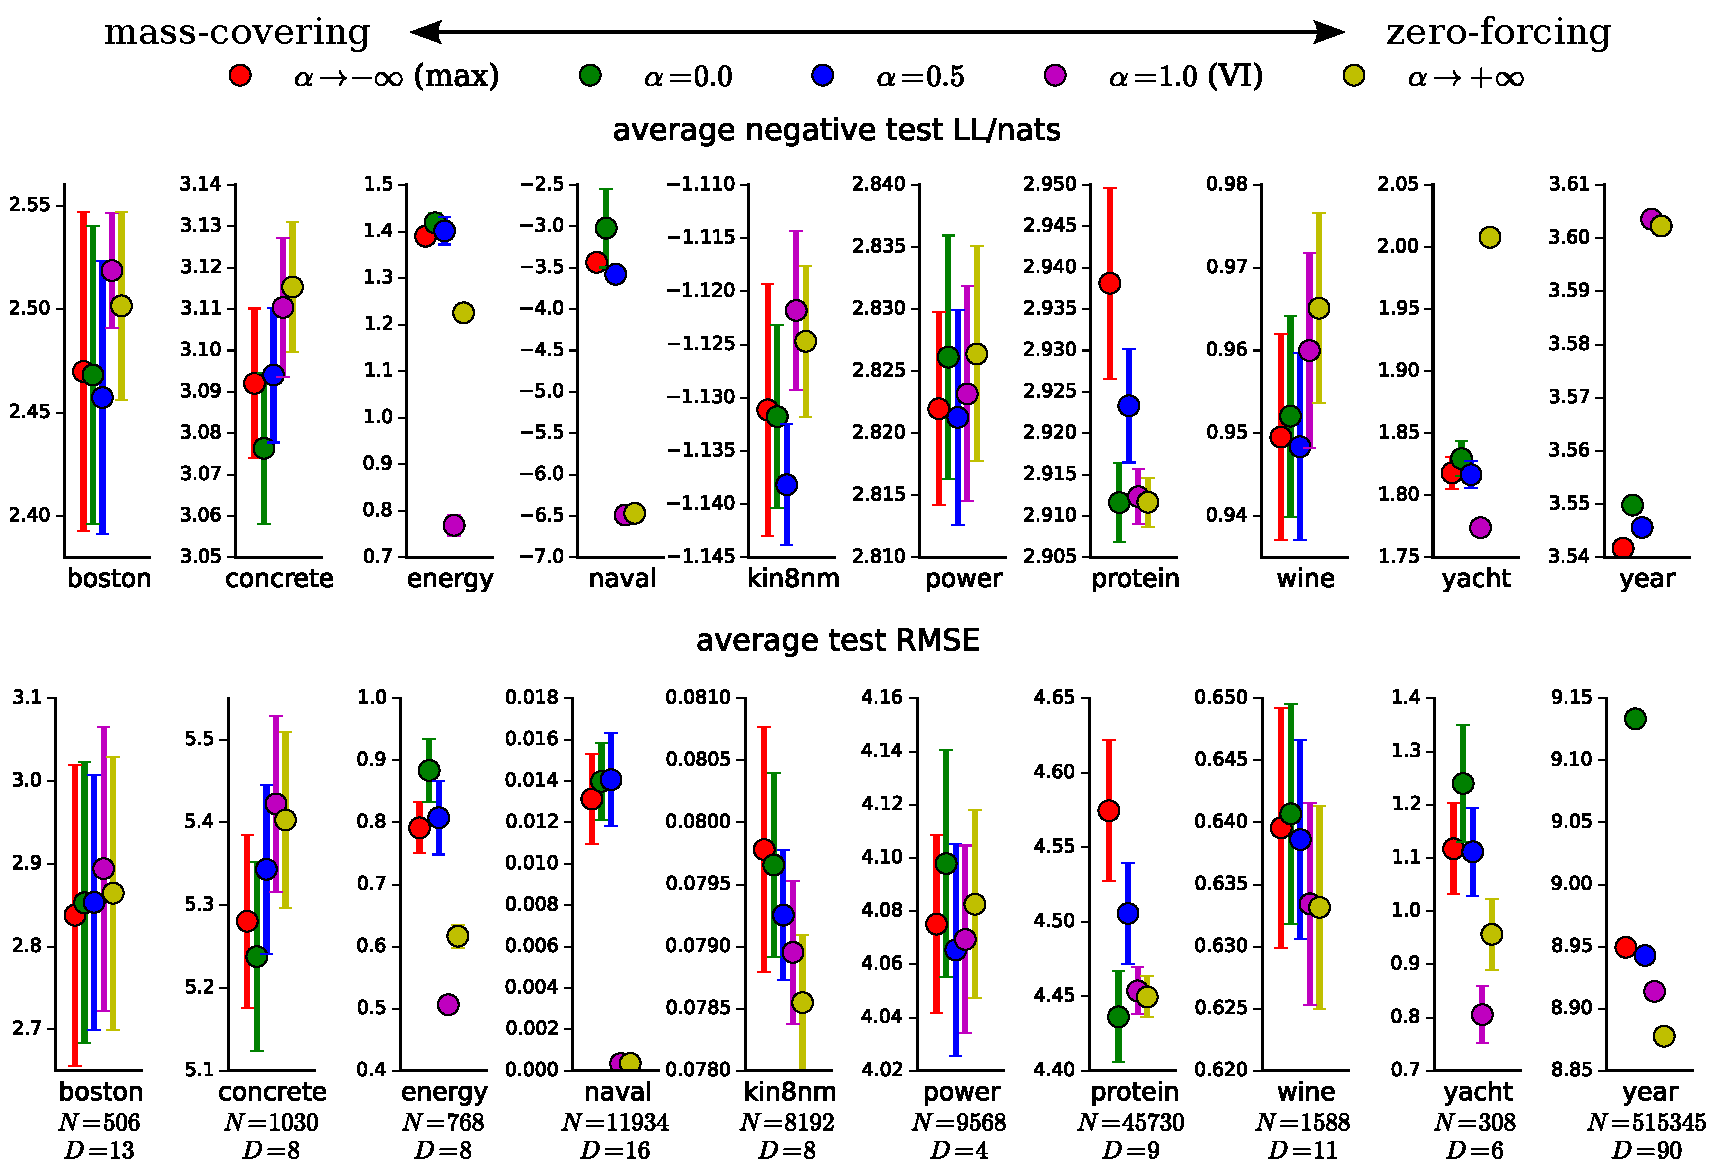
\includegraphics[width=1\linewidth]{Chapter4/vrbound/figs/results_all_bnn}
    \caption{Test LL and RMSE results for Bayesian neural network regression. The lower the better. The error bars show 1-standard deviation across 20 random splits of the data.}
    \label{fig:chap4_vrbound_bnn_results_all}
\end{figure}
%
\begin{figure}
%\begin{table}[ht]
\centering
\captionof{table}{Regression experiment: Average negative test log likelihood/nats}
\label{tab:chap4_vrbound_bnn_ll}
\begin{tabular}{l@{\ica}r@{\ica}r@{\ica}r@{$\pm$}l@{\ica}r@{$\pm$}l@{\ica}r@{$\pm$}l@{\ica}r@{$\pm$}l@{\ica}r@{$\pm$}l@{\ica}}
\hline
\bf{Dataset}&{N}&{D}&\multicolumn{2}{c}{\bf{$\alpha \rightarrow -\infty$}}&\multicolumn{2}{c}{\bf{$\alpha = 0.0$}}&\multicolumn{2}{c}{\bf{$\alpha = 0.5$}}&\multicolumn{2}{c}{\bf{$\alpha = 1.0$ (VI)}}&\multicolumn{2}{c}{\bf{$\alpha \rightarrow +\infty$}}\\
\hline
boston&506&13&2.47&0.08&2.47&0.07&\underline{\textit{2.46}}&\underline{\textit{0.07}}&\textbf{2.52}&\textbf{0.03}&2.50&0.05\\
concrete&1030&8&3.09&0.02&\underline{\textit{3.08}}&\underline{\textit{0.02}}&3.09&0.02&3.11&0.02&\textbf{3.12}&\textbf{0.02}\\
energy&768&8&1.39&0.02&\textbf{1.42}&\textbf{0.02}&1.40&0.03&\underline{\textit{0.77}}&\underline{\textit{0.02}}&1.23&0.01\\
naval&11934&16&-3.43&0.08&\textbf{-3.02}&\textbf{0.48}&-3.58&0.08&\underline{\textit{-6.49}}&\underline{\textit{0.04}}&-6.47&0.09\\
kin8nm&8192&8&-1.13&0.01&-1.13&0.01&\underline{\textit{-1.14}}&\underline{\textit{0.01}}&\textbf{-1.12}&\textbf{0.01}&-1.12&0.01\\
power&9568&4&2.82&0.01&2.83&0.01&\underline{\textit{2.82}}&\underline{\textit{0.01}}&2.82&0.01&\textbf{2.83}&\textbf{0.01}\\
protein&45730&9&\textbf{2.94}&\textbf{0.01}&\underline{\textit{2.91}}&\underline{\textit{0.00}}&2.92&0.01&2.91&0.00&2.91&0.00\\
wine&1588&11&0.95&0.01&0.95&0.01&\underline{\textit{0.95}}&\underline{\textit{0.01}}&0.96&0.01&\textbf{0.97}&\textbf{0.01}\\
yacht&308&6&1.82&0.01&1.83&0.01&1.82&0.01&\underline{\textit{1.77}}&\underline{\textit{0.01}}&\textbf{2.01}&\textbf{0.00}\\
year&515345&90&\underline{\textit{3.54}}&NA&3.55&NA&3.55&NA&\textbf{3.60}&NA&3.60&NA\\
\hline
\multicolumn{3}{c}{\textbf{Average Rank}}&2.80&0.34&3.00&0.45&\textbf{2.20}&\textbf{0.37}&3.20&0.51&3.80&0.39\\
\hline
\end{tabular}
%\end{table}

%\begin{table}[ht]
\centering
\captionof{table}{Regression experiment: Average test RMSE}
\label{tab:chap4_vrbound_bnn_rmse}
\begin{tabular}{l@{\ica}r@{\ica}r@{\ica}r@{$\pm$}l@{\ica}r@{$\pm$}l@{\ica}r@{$\pm$}l@{\ica}r@{$\pm$}l@{\ica}r@{$\pm$}l@{\ica}}
\hline
\bf{Dataset}&{N}&{D}&\multicolumn{2}{c}{\bf{$\alpha \rightarrow -\infty$}}&\multicolumn{2}{c}{\bf{$\alpha = 0.0$}}&\multicolumn{2}{c}{\bf{$\alpha = 0.5$}}&\multicolumn{2}{c}{\bf{$\alpha = 1.0$ (VI)}}&\multicolumn{2}{c}{\bf{$\alpha \rightarrow +\infty$}}\\
\hline
boston&506&13&\underline{\textit{2.84}}&\underline{\textit{0.18}}&2.85&0.17&2.85&0.15&\textbf{2.89}&\textbf{0.17}&2.86&0.17\\
concrete&1030&8&5.28&0.10&\underline{\textit{5.24}}&\underline{\textit{0.11}}&5.34&0.10&\textbf{5.42}&\textbf{0.11}&5.40&0.11\\
energy&768&8&0.79&0.04&\textbf{0.88}&\textbf{0.05}&0.81&0.06&\underline{\textit{0.51}}&\underline{\textit{0.01}}&0.62&0.02\\
naval&11934&16&0.01&0.00&0.01&0.00&\textbf{0.01}&\textbf{0.00}&\underline{\textit{0.00}}&\underline{\textit{0.00}}&0.00&0.00\\
kin8nm&8192&8&\textbf{0.08}&\textbf{0.00}&0.08&0.00&0.08&0.00&0.08&0.00&\underline{\textit{0.08}}&\underline{\textit{0.00}}\\
power&9568&4&4.08&0.03&\textbf{4.10}&\textbf{0.04}&\underline{\textit{4.07}}&\underline{\textit{0.04}}&4.07&0.04&4.08&0.04\\
protein&45730&9&\textbf{4.57}&\textbf{0.05}&\underline{\textit{4.44}}&\underline{\textit{0.03}}&4.51&0.03&4.45&0.02&4.45&0.01\\
wine&1588&11&0.64&0.01&\textbf{0.64}&\textbf{0.01}&0.64&0.01&0.63&0.01&\underline{\textit{0.63}}&\underline{\textit{0.01}}\\
yacht&308&6&1.12&0.09&\textbf{1.24}&\textbf{0.11}&1.11&0.08&\underline{\textit{0.81}}&\underline{\textit{0.05}}&0.96&0.07\\
year&515345&90&8.95&NA&\textbf{9.13}&NA&8.94&NA&8.91&NA&\underline{\textit{8.88}}&NA\\
\hline
\multicolumn{3}{c}{\textbf{Average Rank}}&3.40&0.38&3.70&0.51&3.20&0.31&2.40&0.45&\textbf{2.30}&\textbf{0.38}\\
\hline
\end{tabular}
%\end{table}

       
\end{figure}

We summarise the test negative log-likelihood (LL) and RMSE with standard error (across different random splits except for Year) for selected datasets in Figure \ref{fig:chap4_vrbound_bnn_results_all} and Table \ref{tab:chap4_vrbound_bnn_ll}, \ref{tab:chap4_vrbound_bnn_rmse}. In the tables the best performing results are underlined, while the worse cases are also bold-faced. These results indicate that for posterior approximation problems, the optimal $\alpha$ may vary for different datasets (although for Boston and Power the performances are very similar). 
%

It can be particularly tricky to approximate the posterior distribution of the weight matrices for a neural network. Since one can obtain the same output by swapping the positions of two hidden units and adjusting the corresponding in- and out-going weights, there exist symmetric modes in the exact posterior of the weight matrices. In this case mass-covering can be harmful, e.g.~for Naval and Energy datasets, methods with $\alpha < 1.0$ values seem to be under-performing, not only for predictive error but also for test log-likelihood measure. 
But still, we observed two major trends. Zero-forcing/mode-seeking methods tend to focus on improving the predictive error. Mass-covering methods, on the other hand, returns better test log-likelihood, which has been shown empirically to be correlated with the quality of the approximated uncertainty estimate \citep{hernandez-lobato:pbp2015, gal:uncertainty2016, depeweg:bnn_rl2016}. In particular VI returns lower test log-likelihood for most of the datasets. Furthermore, $\alpha = 0.5$ produced overall good results for both test LL and RMSE, possibly because the skew symmetry is centred at $\alpha = 0.5$ and the corresponding divergence is the only symmetric distance measure in the family. Future work should develop algorithms to automatically select the best $\alpha$ values, although a naive approach could use validation sets. 

\subsection{Variational auto-encoders}

The second experiments considers variational auto-encoders for unsupervised learning. We mainly compare three approaches: VAE ($\alpha = 1.0$), IWAE ($\alpha = 0$), and VR-max ($\alpha = -\infty$), which are implemented upon the publicly available code.\footnote{\url{https://github.com/yburda/iwae}}
%
Four datasets are considered: Frey Face\footnote{\url{http://www.cs.nyu.edu/~roweis/data.html}} (with 10-fold cross validation), Caltech 101 Silhouettes\footnote{\url{https://people.cs.umass.edu/~marlin/data.shtml}}, MNIST\footnote{\url{http://yann.lecun.com/exdb/mnist/}} and OMNIGLOT\footnote{\url{https://github.com/brendenlake/omniglot}}. The VAE model has $L=1, 2$ stochastic layers with deterministic layers stacked between.  The detailed numbers of stochastic layers $L$, number of hidden units, and the activation function are summarised in Table \ref{tab:vae_arch}. The prefix of the number indicates whether this layer is \textbf{d}eterministic or \textbf{s}tochastic, e.g.~d500-s200 stands for a neural network with one deterministic layer of 500 units followed by a stochastic layer of 200 units. For Frey Face data we train the models using learning rate 0.0005 and mini-batch size 100. For MNIST and OMNIGLOT we reuse the settings from \cite{burda:iwae2016}: the training process runs for $3^i$ passes with learning rate $0.0001 \cdot 10^{-i/7}$ for $i = 0, ..., 7$, and the batch size is 20. For Caltech Silhouettes we use the same settings as MNIST and OMNIGLOT except that the training proceeded for $\sum_{i=0}^7 2^i = 255$ epochs. We reproduce the IWAE experiments to obtain a fair comparison, since the results in the original publication \citep{burda:iwae2016} mismatches those evaluated on the publicly available code.
%

\begin{table}[!ht]
\centering
\captionof{table}{Network architecture of tested VAE algorithms.}
\label{tab:vae_arch}
\begin{tabular}{lccccc}
\hline
\bf{Dataset}&$L$&architecture&activation&probability type (p/q)\\
\hline
Frey Face&1& d200-d200-s20&softplus&Gaussian/Gaussian\\
\hline
Caltech 101& 1&d500-s200&tanh&Bernoulli/Gaussian\\
\hline
MNIST \& & 1&d200-d200-s50&tanh&Bernoulli/Gaussian\\
OMNIGLOT     & 2&d200-d200-s100-d100-d100-s50&tanh&Bernoulli/Gaussian\\
\hline
\end{tabular}
\end{table}

%

\begin{figure}
\begin{minipage}{0.6\linewidth}

%\begin{table}[t]
\centering
%\caption
\captionof{table}{ Average Test log-likelihood. Results for VAE on MNIST and OMNIGLOT are collected from \cite{burda:iwae2016}.}
\label{tab:vae_ll}
\begin{tabular}{lccccc}
\toprule
\bf{Dataset}&$L$&$K$&\bf{ VAE }&\bf{ IWAE }&\bf{ VR-max }\\
\hline
Frey Face&1&5&1322.96&\bf{1380.30}&1377.40\\
($\pm$ std. err.)& & &$\pm$10.03&\bf{$\pm$4.60}&$\pm$4.59 \\
\hline
Caltech 101& 1& 5&-119.69&\bf{-117.89}&-118.01\\
Silhouettes&  &50&-119.61&-117.21&\bf{-117.10}\\
\hline
MNIST& 1&5 &-86.47&\bf{-85.41}&-85.42\\
     &  &50&-86.35&\bf{-84.80}&-84.81\\
     & 2&5 &-85.01&\bf{-83.92}&-84.04\\
     &  &50&-84.78&\bf{-83.05}&-83.44\\
\hline
OMNIGLOT & 1&5 &-107.62&\bf{-106.30}&-106.33\\
		 & 1&50&-107.80&\bf{-104.68}&-105.05\\
		 & 2&5 &-106.31&\bf{-104.64}&-104.71\\
		 & 2&50&-106.30&\bf{-103.25}&-103.72\\
\bottomrule
\end{tabular}
%\end{table}

\end{minipage}
\hfill
\begin{minipage}{0.35\linewidth}
\centering
 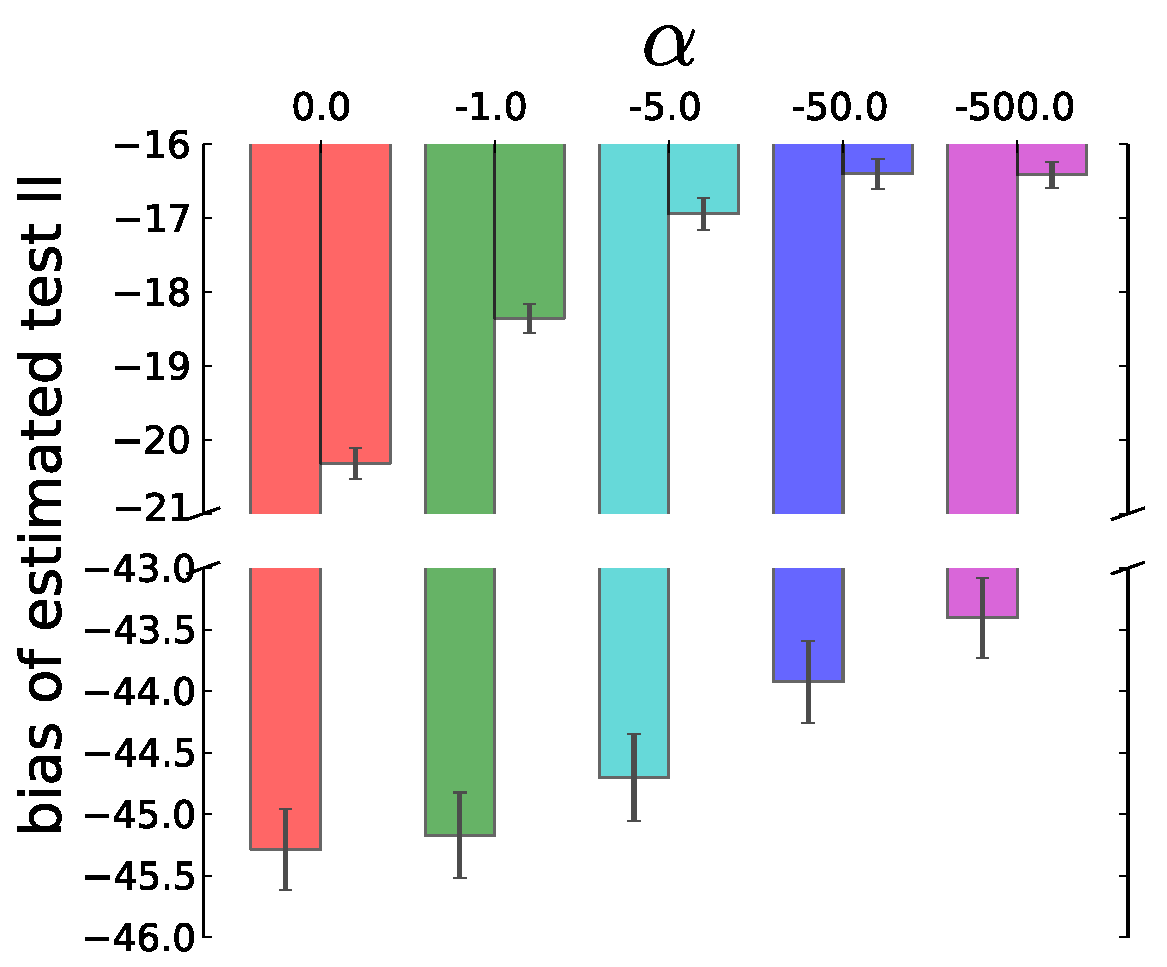
\includegraphics[width=1.00\linewidth]{Chapter4/vrbound/figs/bias_estimate.pdf} 
 \captionof{figure}{Bias of sampling approximation to. Results for $K=5, 50$ samples are shown on the left and right, respectively.}
 \label{fig:vae_bias}
\end{minipage}
\end{figure}
%
\begin{figure*}[!ht]
 \centering
 \subfigure[Log of ratio $R = w_{max} / (1 - w_{max})$]{
 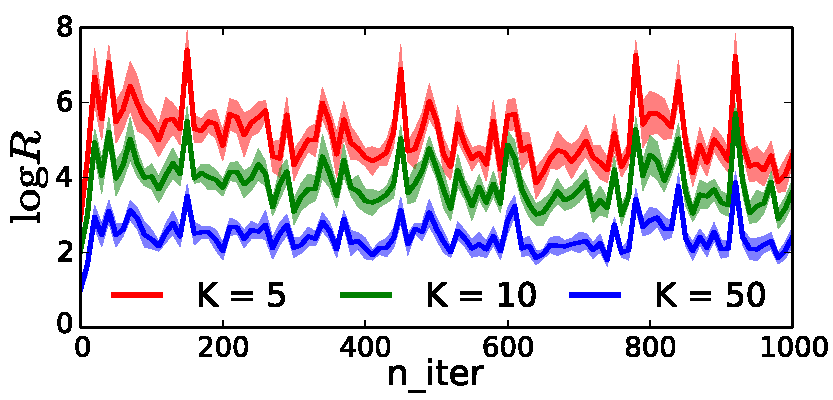
\includegraphics[width=0.37\linewidth]{Chapter4/vrbound/figs/weight_ratio.pdf}
 \label{fig:weight_ratio}}
 \hspace{0.4in}
 \subfigure[Weights of samples.]{
 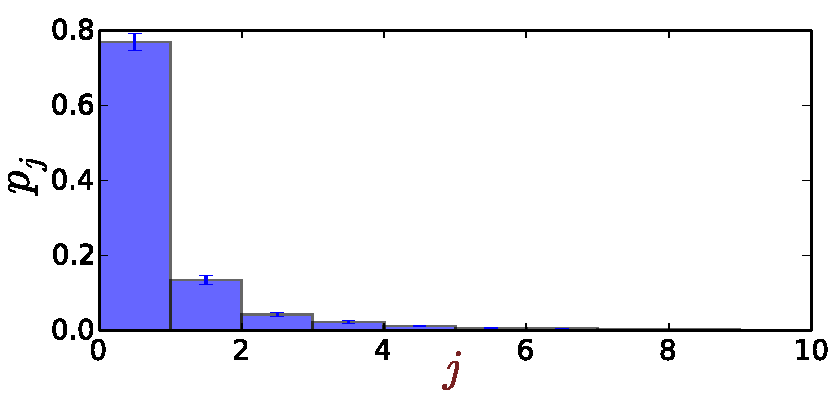
\includegraphics[width=0.37\linewidth]{Chapter4/vrbound/figs/weight_distribution.pdf}
 \label{fig:weight_distribution}}
 \caption{Importance weights during training, see main text for details. Best viewed in colour.}
\end{figure*}

We report test log-likelihood results in Table \ref{tab:vae_ll} by computing $\log p(\bm{x}) \approx \hat{\mathcal{L}}_{0, 5000}(q; \bm{x})$ following \cite{burda:iwae2016}. We also present some samples from the VR-max trained auto-encoders in Figure \ref{fig:vae_samples}.
%
\begin{figure}
 \centering
  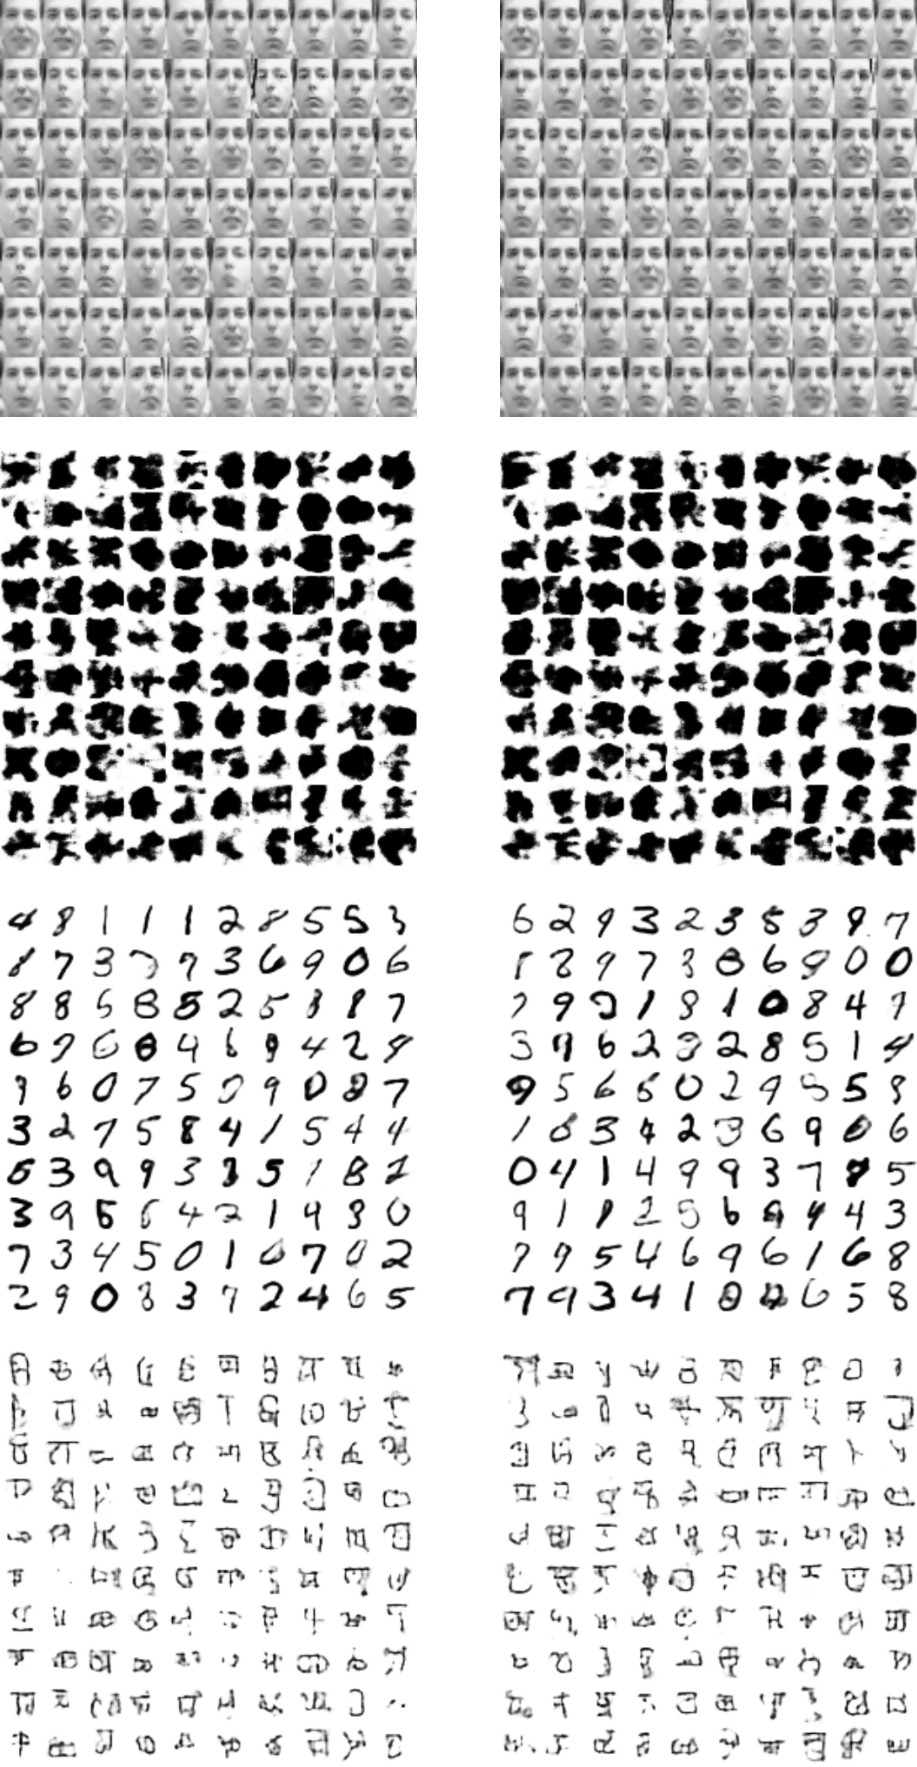
\includegraphics[width=0.6\linewidth]{Chapter4/vrbound/figs/vae_samples.pdf}
  \caption{Sampled images from the the best models trained with IWAE (left) and VR-max (right).}
  \label{fig:vae_samples}
\end{figure}
%
Overall VR-max is almost indistinguishable from IWAE. Other positive alpha settings (e.g.~$\alpha = 0.5$) return worse results, e.g. $1374.64\pm5.62$ for Frey Face and $-85.50$ for MNIST with $\alpha = 0.5$, $L=1$ and $K=5$. These worse results for $\alpha > 0$ indicate the preference of getting tighter approximations to the likelihood function for MLE problems. Small negative $\alpha$ values (e.g.~$\alpha = -1.0, -2.0$) return better results on different splits of the Frey Face data, and overall the best $\alpha$ value is dataset-specific.\footnote{Since presentation of this work at NIPS 2016, \cite{bui:dgm2016} revisited this idea with slightly different architecture set-up, and showed that $\alpha \neq 0$ values are usually favoured over the IWAE approach. }

VR-max's success might be explained by the tightness of the bound. To evaluate this, we compute the VR bounds on $100$ test datapoints using the 1-layer VAE trained on Frey Face, with $K=\{5, 50\}$ and $\alpha \in \{0, -1, -5, -50, -500 \}$. Figure \ref{fig:vae_bias} presents the estimated gap $\hat{\mathcal{L}}_{\alpha, K} - \hat{\mathcal{L}}_{0, 5000}$. The results indicates that $\hat{\mathcal{L}}_{\alpha, K}$ provides a lower-bound, agreeing with the theoretical results presented in Section \ref{sec:chap4_vrbound_sampling}, and that gap is narrowed as $\alpha \rightarrow -\infty$. Also increasing $K$ provides improvements. The standard error of estimation is almost constant for different $\alpha$ (with $K$ fixed), and is negligible when compared to the MC approximation bias.

%
Another explanation for VR-max's success is that, the sample with the largest normalised importance weight $w_{max}$ dominates the contributions of all the gradients.
This is confirmed by tracking $R = \frac{w_{max}}{1 - w_{max}}$ during training on Frey Face (Figure \ref{fig:weight_ratio}). Also Figure \ref{fig:weight_distribution} shows the $10$ largest importance weights from $K=50$ samples in descending order, which exhibit an exponential decay behaviour, with the largest weight occupying more than $75\%$ of the probability mass. This means, the IWAE algorithm is not efficient in terms of sample efficiency, since the learning signal from back-propagation is dominated by the gradients computed on the particle with the largest weight.
%
It also indicates that, VR-max can provide a fast approximation to IWAE when tested on CPUs or multiple GPUs with high communication costs. Indeed our numpy implementation of VR-max achieves up to a 3 times speed-up compared to IWAE (9.7s vs.~29.0s per epoch, tested on Frey Face data with $K = 50$ and batch size $M = 100$, CPU info: Intel Core i7-4930K CPU @ 3.40GHz). However this speed advantage is less significant when the gradients can be computed very efficiently on a single GPU.
\section{Summary}
We have introduced the variational R{\'e}nyi bound and an associated optimisation framework. We have shown the richness of the new family, not only by connecting to existing approaches including VI/VB, SEP, BB-$\alpha$, VAE and IWAE, but also by proposing the VR-max algorithm as a new special case. Empirical results on Bayesian neural networks and variational auto-encoders indicate that VR bound methods are widely applicable and can obtain state-of-the-art results.
%
%
Future work will focus on both experimental and theoretical aspects. Theoretical work will study the interaction of the biases introduced by MC approximation and datapoint sub-sampling. Also a quantitative analysis of the MC approximation bias will be very useful, especially for model selection. 

%\section{Free-energy construction with decoupling and constraint relaxations}
%\label{sec:constraint_relaxation_all}
%\subsection{EP energy: a primal-dual story}
\label{sec:chap2_ep_energy}

EP has been criticised for not having convergence guarantees and instead being a heuristic for posterior approximation. On the other hand, it has been shown to have superior performance compared to VI on a variety of tasks, e.g.~Gaussian Process classification \citep{kuss:gpep2005}. To understand these seemingly contradicting observations, here we provide an energy minimisation view of EP,\footnote{material based on my NIPS 2016 approximate inference workshop abstract, see publication page.} and discuss why EP could potentially lead to better approximations, and why it is difficult to prove the convergence of EP. Similar derivations are also available in \citet{yedidia:bethe2001, heskes:ep2002, minka:divergence2005, opper:ec2005, wainwright:graphical2008}, and some extensions to handling latent variable models are provided in appendix \ref{sec:appendix_relaxation}.

To streamline the notation, we consider approximating the intractable posterior $p(\mparam|\mathcal{D}) = \frac{1}{Z} p_0(\mparam) \prod_{n=1}^N p(\bm{x}_n|\mparam)$ as a running example. In this case we denote $\tilde{f}_n(\mparam) = p(\bm{x}_n|\mparam)$ and leave the prior $p_0(\mparam)$ as it is. Using this notation we again write down the objective function of Variational inference (VI) called the \emph{variational free energy} (VFE) \citep{jordan:vi1999, beal:vi2003}:
\begin{equation}
\min_{q \in \mathcal{Q}} \mathrm{KL}[q||p] \Leftrightarrow \min_{q \in \mathcal{Q}} \mathcal{F}_{\text{VFE}}(q) = \mathbb{E}_{q} \left[ \log q(\mparam) - \log p_0(\mparam) - \sum_{n=1}^N \log \tilde{f}_n(\mparam) \right].
\label{eq:ep_section_vfe}
\end{equation}

\subsubsection{From VFE to Bethe Free Energy}
\label{sec:vfe_to_bethe}

First we make use of the additivity of logarithm to rewrite an equivalent optimisation problem (recall that $\mathcal{P}$ is the space of all probability distributions):
\begin{equation}
\begin{aligned}
\min_{q \in \mathcal{Q}} \mathcal{F}_{\text{VFE}}(q)
&= \min_{q \in \mathcal{Q}} \mathrm{KL}[q||p_0] - \sum_n \mathbb{E}_{q} \left[ \log \frac{p_0(\mparam) \tilde{f}_n(\mparam)}{q(\mparam)} \right] - N \mathrm{KL}[q || p_0] \\
& = \min_{ q \in \mathcal{Q}, \{ \tilde{p}_n \in \mathcal{P} \} } (1 - N) \mathrm{KL}[q||p_0] - \sum_n \mathbb{E}_{\tilde{p}_n} \left[ \log \frac{p_0(\mparam) \tilde{f}_n(\mparam)}{\tilde{p}_n(\mparam)} \right] \\ 
& \quad \quad \quad \quad \text{ subject to } \tilde{p}_n = q, \forall n. 
\end{aligned}
\label{eq:vi_constrained}
\end{equation}
%
Here in the first line we added $N$ copies of $\mathrm{KL}[q || p_0]$ to the VFE and subtracted the same, and in the second line we \emph{decoupled} the tilted distribution $\tilde{p}_n$ from $q$ by introducing equality constraints. This means the above optimisation has the same fixed points as minimising VFE. The constraints can be \emph{relaxed} to matching all the moments $\mathbb{E}_{\tilde{p}_n}[\mparam^{k}] = \mathbb{E}_q[\mparam^k]$ for $k \in \mathbb{N}$,\footnote{Having the same moments for $p$ and $q$ does not imply having the same \emph{moment generating function}.} and a further crude relaxation suggests moment matching just for the first $K$ moments\footnote{The zeroth moment matching constraint is replaced by the constraint that $\tilde{p}_n$ integrates to 1.}
$\mathbb{E}_{\tilde{p}_n}[\mparam^{k}] = \mathbb{E}_q[\mparam^k], k = 1, 2, ..., K$.
%
In the following we use a vectorial function $\bm{\Phi}(\mparam)$ to summarise these constraints as $\mathbb{E}_{\tilde{p}_n}[\bm{\Phi}] = \mathbb{E}_q[\bm{\Phi}]$, where as an example for Gaussian EP: $\bm{\Phi}(\mparam) = [\mparam, \mparam \mparam^T]$. In general $\bm{\Phi}$ can contain any polynomial terms or other basis functions. This relaxation returns the following constrained optimisation problem:
%
\begin{equation}
\begin{aligned}
 \min_{ q \in \mathcal{Q}, \{ \tilde{p}_n \in \mathcal{P} \} } \mathcal{F}_{\text{Bethe}}( \{ \tilde{p}_n \}, q) \quad \text{subject to } \mathbb{E}_{\tilde{p}_n}[\bm{\Phi}] = \mathbb{E}_q[\bm{\Phi}], \forall n, \\
\mathcal{F}_{\text{Bethe}}( \{ \tilde{p}_n \}, q) =  (1 - N) \mathrm{KL}[q||p_0] - \sum_n \mathbb{E}_{\tilde{p}_n} \left[ \log \frac{p_0(\mparam) \tilde{f}_n(\mparam)}{\tilde{p}_n(\mparam)} \right].
\end{aligned}
\label{eq:bethe}
\end{equation}
$\mathcal{F}_{\text{Bethe}}( \{ \tilde{p}_n \}, q)$ is the \emph{Bethe free energy} \citep{bethe:energy1935, yedidia:bethe2001} that is usually presented in the context of probabilistic graphical models and belief propagation. Below we show how to derive its dual form that is usually discussed in EP literature \citep{minka:ep_energy2001, opper:ec2005, seeger:ep2005}. 

\vspace{1em}
\begin{tcolorbox}
\textbf{Remark} (Tom Minka's original note)\textbf{.}
\cite{minka:ep_energy2001} formulated (\ref{eq:bethe}) as a minimax problem ($\min_{\{\tilde{p}_n \}} \max_{q}$) instead which seems questionable to me.  First (\ref{eq:bethe}) relaxes the constraints in (\ref{eq:vi_constrained}), meaning both should have the same optimisation direction. Then since (\ref{eq:vi_constrained}) just decouples VFE (\ref{eq:ep_section_vfe}) with equality constraints, it should be a pure minimisation and has the same stationary points. For graphical models the Bethe free energy optimisation problem is formulated as a pure minimisation problem like above (\ref{eq:bethe}), e.g.~in \cite{heskes:bp_fixed_point2002, wainwright:graphical2008} but also interestingly in pages 3-4 of \cite{minka:ep_energy2001}. On the other hand, Minka's derivation of the dual energy differs from solving the Lagrangian and does not require the minimax assumption of the primal problem. 
\end{tcolorbox}

\subsubsection{From Bethe to EP: a dual form representation}
\label{sec:ep_fixed_points}
We provide a derivation in a similar way as \cite{heskes:bp_fixed_point2002}, starting from a note on the KL duality\footnote{We include this step in order to connect to the EP energy with optimisation arguments all in the dual space.}
\begin{equation}
 -\mathrm{KL}[q||p_0] = \min_{\bm{\lambda}_{q}(\mparam)} - \mathbb{E}_q[\lambda_q(\mparam)] + \log \mathbb{E}_{p_0} \left[ \exp [\lambda_q(\mparam)] \right],
 \label{eq:kl_duality}
\end{equation}
with $\lambda_q(\mparam)$ a function to be specified later on. This duality is in the same spirit as deriving convex conjugate function for the log partition function of an exponential family distribution (see Proposition \ref{prop:chap2_expfam}), if viewing $p_0(\mparam)$ as the base measure.
The equality is achieved by $q(\mparam) \propto p_0(\mparam) \exp[\lambda_q(\mparam)]$.
%
Substitution into (\ref{eq:bethe}) then yields a transformed energy that we denoted as $\mathcal{F}_{\text{Bethe}}(\{ \tilde{p}_n \}, q, \lambda_q(\mparam))$.
%
\begin{equation}
\begin{aligned}
\mathcal{F}_{\text{Bethe}}(\{ \tilde{p}_n \}, q, \lambda_q(\bm{\theta})) = (1 - N) \mathbb{E}_q[\lambda_q(\bm{\theta})] + (N - 1) \log \mathbb{E}_{p_0} \left[ \exp [\lambda_q(\bm{\theta})] \right] \\
- \sum_n \mathbb{E}_{\tilde{p}_n} \left[ \log \frac{p_0(\bm{\theta}) \tilde{f}_n(\bm{\theta})}{\tilde{p}_n(\bm{\theta})} \right].
\label{eq:bethe_energy_transformed}
\end{aligned}
\end{equation}

%
Denote $\bm{\lambda}_{-n}$ as the Lagrange multiplier for moment matching and $\nu, \nu_n$ for the normalisation constraints of $q$ and $\tilde{p}_n$, respectively. This returns the following Lagrangian
\begin{equation}
\begin{aligned}
 \min_{q, \{ \tilde{p}_n \}, \lambda_q(\bm{\theta}) } \max_{\{ \bm{\lambda}_{-n}, \nu_n, \nu \} } \mathcal{F}_{\text{Bethe}}( \{ \tilde{p}_n \}, q, \lambda_q(\bm{\theta})) + \sum_n \bm{\lambda}_{-n}^{T}(\mathbb{E}_q[\bm{\phi}] - \mathbb{E}_{\tilde{p}_n}[\bm{\phi}]) \\
 + \sum_n \nu_n \left( \int \tilde{p}_n(\bm{\theta}) d\bm{\theta} - 1 \right) + \nu \left( \int q(\bm{\theta}) d\bm{\theta} - 1 \right) .
\end{aligned} 
\label{eq:bethe_lagranrian}
\end{equation}
Solving the fixed points for $\tilde{p}_n$ and $\nu_n$ returns 
$$
\tilde{p}_n(\mparam) = \frac{1}{Z_n} p_0(\mparam)\tilde{f}_n(\mparam) \exp \left[ \bm{\lambda}_{-n}^T \bm{\Phi}(\mparam) \right],
$$
where the normalising constant is $$Z_n = \int p_0(\mparam) \tilde{f}_n(\mparam) \exp \left[ \bm{\lambda}_{-n}^T \bm{\Phi}(\mparam) \right] d \mparam.$$ 
%
Also it is straight-forward to evaluate the fixed point condition for $q$: $$(N - 1) \lambda_q(\mparam) = \sum_n \bm{\lambda}_{-n}^T \bm{\Phi}(\mparam) + \nu.$$
We explicitly specify $\lambda_q(\mparam) = \bm{\lambda}_q^T \bm{\Phi}(\mparam) + \nu$ w.l.o.g., also the constant $\nu$ can be dropped since exponential family distributions are translation invariant to constants.
%
Importantly, substituting $\tilde{p}_n$ back to (\ref{eq:bethe_lagranrian}) and enforcing the fixed point condition for $q$ yields the \emph{EP energy} \citep{minka:ep_energy2001}:
\begin{equation}
\begin{aligned}
\min_{\bm{\lambda}_q} \max_{\{ \bm{\lambda}_{-n} \} } \mathcal{F}_{\text{EP}}(\bm{\lambda}_q, \{ \bm{\lambda}_{-n} \} ) =  (N - 1) \log \mathbb{E}_{p_0} \left[ \exp [\bm{\lambda}_q^T \bm{\Phi}(\mparam)] \right] - \sum_n \log Z_n,\\
 \text{subject to } (N - 1) \bm{\lambda}_q = \sum_n \bm{\lambda}_{-n}.
\end{aligned}
\label{eq:ep_energy}
\end{equation}
Notice now the optimisation problem over $q$ is dropped since (\ref{eq:ep_energy}) does not depend on it. To obtain the approximate posterior back, we make use of the tightness of the KL duality, and define 
$$q(\mparam) = \frac{1}{Z_q} p_0(\mparam) \exp \left[ \bm{\lambda}_q^T \bm{\Phi}(\mparam) \right],  \quad \log Z_q = \log \mathbb{E}_{p_0} \left[ \exp [\bm{\lambda}_q^T \bm{\Phi}(\mparam)] \right].$$
%
The expectation consistent approximate inference (EC) algorithm \citep{opper:ec2005} is a special case with $p_0(\mparam) \propto 1$ and $N = 2$. 

\subsubsection{EP as a fix point iteration method for solving the dual problem}

EP \citep{minka:ep2001} proposes parametrising the (natural parameters of) local approximating factors $f_n \approx \tilde{f}_n$ instead of the approximate posterior $q$, with the goal of $f_n$ capturing the effect of $\tilde{f}_n(\mparam)$ on the exact posterior, by defining $f_n(\mparam) = \exp [\bm{\lambda}_n^T \bm{\Phi}(\mparam)]$, $\bm{\lambda}_n = \bm{\lambda}_q - \bm{\lambda}_{-n}$. Thus by construction the constraint in (\ref{eq:ep_energy}) is automatically satisfied: $\bm{\lambda}_q = \sum_n \bm{\lambda}_n$ and $\bm{\lambda}_{-n} = \sum_{m \neq n} \bm{\lambda}_m$.
%
Then EP runs a fixed point iteration algorithm to find a stationary point for $\{ \bm{\lambda}_n \}_{n=1}^N$. More specifically the gradient of (\ref{eq:ep_energy}) w.r.t.~the local parameter $\bm{\lambda}_n$ is 
\begin{equation}
\nabla_{\bm{\lambda}_n} \mathcal{F}_{\text{EP}} = (N-1) \mathbb{E}_{q} [ \bm{\Phi}(\mparam) ] - \sum_{m \neq n} \mathbb{E}_{\tilde{p}_m} [ \bm{\Phi}(\mparam) ].
\end{equation} 
Zeroing the above gradient for all $\bm{\lambda}_n$ results in the fixed point condition
$$\mathbb{E}_q[\bm{\Phi}(\mparam)] = \mathbb{E}_{\tilde{p}_n}[ \bm{\Phi}(\mparam) ], \quad \forall n,$$
which motivates the moment matching update (\ref{eq:chap2_ep_moment_matching}) in EP.

\subsubsection{A pictorial view on why EP can be better than VI}
Folk wisdom suggests that EP, if it convergences, often provide more accurate approximations to the target distribution when compared with VI. This observation is explained pictorially in Figure \ref{fig:chap2_ep_vi_comparison}. 
%
Recall that both algorithms can be viewed as minimising the Bethe free energy under constraints: for VI the constraints are equality constraints $q = \tilde{p}_n$, whereas EP instead uses moment matching constraints $\mathbb{E}_q[\bm{\Phi}] = \mathbb{E}_{\tilde{p}_n}[\bm{\Phi}]$. In an augmented space $\mathcal{P}^{N+1}$, the search space of VI $\{ (q, \tilde{p}_n): q = \tilde{p}_n, q \in \mathcal{Q} \}$ is contained in the search space of EP $ \{ (q, \tilde{p}_1, ..., \tilde{p}_N): q \in \mathcal{Q}, \mathbb{E}_{\tilde{p}_n}[\bm{\Phi}] = \mathbb{E}_q[\bm{\Phi}] \}$, and can be of much smaller dimensions (e.g.~the green line segment versus the blue region as shown in the Figure \ref{fig:chap2_ep_vi_comparison}). Therefore if EP converges, then it is more likely to find a better minimum compared to VI. Empirical evidence also suggests that constrained Bethe free-energy evaluated at a fixed point is often a better approximation to the (negative log) marginal likelihood.

\begin{figure}
\centering
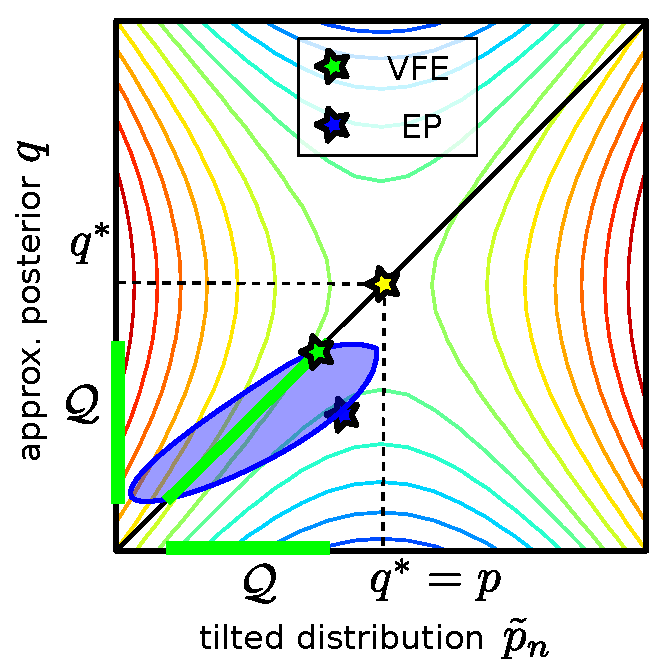
\includegraphics[width=0.4\linewidth]{Chapter2/ep/energy.pdf}
\caption{EP versus VI as constrained energy optimisation problems, visualised by projecting the energy surface from the augmented space $\mathcal{P}^{N+1}$ to $\mathcal{P}^{2}$. Here the slash line across the space represents the subspace $\{ (q, \tilde{p}_n): q = \tilde{p}_n \}$, and the search space for VI (the green segment) is contained in the EP candidate set (the blue region). The stars indicate the optimal solutions returned by the exact (in yellow) and the approximate inference algorithms (green/blue). See main text for details.}
\label{fig:chap2_ep_vi_comparison}
\end{figure}

\subsubsection{Criticisms for EP's iterative update}
%
The above fixed point iteration update has no convergence guarantee, which is one of the drawbacks of EP. The reason is that EP solves the dual problem of constrained Bethe free energy minimisation, and that dual problem turns out to be a minimax optimisation problem with constraints. Indeed, a double-loop algorithm \citep{heskes:ep2002} should be applied to (\ref{eq:ep_energy}) if convergence is required. However in practice such a double-loop method has been shown to be much slower than EP. Also disappointedly, even when the exact posterior is contained in $\mathcal{Q}$, EP is not guaranteed to return it. Similar problems exist for belief propagation when the graph contains many loops, or when the relaxed polytope is not \emph{tight} \citep{wainwright:graphical2008}.

%\hl{Another myth about EP is the choice of using fixed point update instead of gradient descent for the local parameters. Here it should be emphasised that the optimisation aims to find a \emph{saddle point} rather than a local minimum/maximum of the energy function. Since it is a minimisation problem for $\bm{\lambda}_q$ and maximisation problem for $\bm{\lambda}_{-n}$, is is also unclear to determine the optimisation problem for the local parameters $\bm{\lambda}_n$. Finally there exists no proof that the EP energy is upper or lower bounded, i.e. the existence of minimum/maximum is unclear as well. All the above situations make the analysis of gradient descent convergence very difficult.}


\subsubsection{From VFE to power EP}
\label{sec:vfe_to_pep}
We now extend the above approach to power EP \citep{minka:powerep2004} which is a new contribution, although fairly straightforward. This procedure includes one modification to the Bethe free energy. Assume for each factor $\tilde{f}_n$ a power value $\alpha_n \neq 0$ is associated, with $\bm{\alpha} = (\alpha_1, ..., \alpha_N)$ and $\sum_n \frac{1}{\alpha_n} \neq 1$. Then the Bethe free energy with moment matching constraints is modified to:
\begin{equation}
\mathcal{F}_{\bm{\alpha}}(q, \{ \tilde{p}_n \}) = \left( 1 - \sum_n \frac{1}{\alpha_n} \right) \mathrm{KL}[q||p_0] - \sum_{n=1}^N \frac{1}{\alpha_n} \mathbb{E}_{\tilde{p}_n} \left[ \log \frac{p_0(\mparam) \tilde{f}_n(\mparam)^{\alpha_n}}{\tilde{p}_n(\mparam)} \right].
\label{eq:alpha_bethe}
\end{equation}
%
Similar to the derivation of (\ref{eq:vi_constrained}), here we first added and subtracted $(\sum_n \frac{1}{\alpha_n})$ copies of $\mathrm{KL}[q||p_0]$, then decoupled $\tilde{p}_n$ from $q$, and relaxed the equality constraints to moment matching. Calculations following Section \ref{sec:ep_fixed_points} also reveal the change of the fixed point condition for $q$ to $(\sum_n \frac{1}{\alpha_n} - 1) \bm{\lambda}_q = \sum_n \frac{1}{\alpha_n} \bm{\lambda}_{-n}$. Define $q$ as an exponential family distribution with natural parameter $\bm{\lambda}_q$ as before, and $\bm{\lambda}_n = (\bm{\lambda}_q - \bm{\lambda}_{-n}) / \alpha_n$. We arrive at the power EP objective:
\begin{equation}
\left( \sum_n \frac{1}{\alpha_n} - 1 \right) \log Z_q - \sum_n \frac{1}{\alpha_n} \log \int p_0(\mparam) \tilde{f}_n(\mparam)^{\alpha_n} \exp \left[ (\bm{\lambda}_q - \alpha_n \bm{\lambda}_n)^T \bm{\Phi}(\mparam) \right] d \mparam.
\label{eq:pep_energy}
\end{equation}
The iterative process also enforces $\bm{\lambda}_q = \sum_n \bm{\lambda}_n$.  \cite{minka:divergence2005} showed that (\ref{eq:pep_energy}) becomes an upper-bound of $\log Z$ when $\alpha_n > 0$ and $\sum_n \frac{1}{\alpha_n} < 1$. On the other hand, taking $\alpha_n \rightarrow 0, \forall n$ recovers $\mathcal{F}_{\text{VFE}}$ but now the $q$ distribution is restricted to have an exponential family form.
%\input{Chapter4/constraint/bbalpha}
%\input{Chapter4/constraint/distributed}
%\input{Chapter4/constraint/lvm}
%\input{Chapter4/constraint/sequential}
%
%\section{Derivations and proofs}
%\label{sec:proofs_chap4}
%\input{Chapter4/proofs/details_vrbound}

\vspace{3em}
{\Large
\noindent \hrulefill \hspace{0.2cm} \raisebox{-4pt}[10pt][10pt]{\decofourleft ~  \decosix ~ \decofourright} \hspace{0.1cm} \hrulefill
\vspace{2em}
}

This ends the first part of the thesis, which has reviewed existing variational methods (Chapter \ref{chap:background}), and proposed two unifying frameworks for both algorithmic (Chapter \ref{chap:factor_tying}) and optimisation objective (Chapter \ref{chap:vrbound}) aspects. Experiments on Bayesian deep learning tasks also proved the successfulness of our efforts, on pushing variational algorithms towards wider applicability (far beyond conjugate models) and better scalability to ``big data, big models''. I do admit that, however, the lack of theoretically rigorous selection of approximate inference algorithms is one of the imperfections of the analysis presented here. 
%
Indeed, a guide on choosing the optimal inference method are needed for practitioners when applying the framework to their applications, which will be one of my research directions in the future.

So far we only studied different optimisation procedures assuming a given approximating distribution family (mean-field Gaussians in the empirical results), which is just one side of the story for approximate inference. The whole picture for this huge subject will never be comprehensive without discussing the other side, i.e.~the construction of $q$ distributions. In the second part of the thesis ``wild approximate inference'', I will revisit the fundamental questions in approximate inference, providing my point of view on the principles of approximate distribution design, and present one of the algorithms I developed during my PhD following these principles.


